\documentclass[11pt,a4paper]{article}
\usepackage[margin=23mm,headheight=15pt,footskip=12mm]{geometry}
\usepackage{fontspec}
\IfFileExists{fonts/NotoSansCJKkr-Regular.otf}{
\setmainfont{NotoSansCJKkr-Regular.otf}[Path=fonts/,BoldFont=NotoSansCJKkr-Bold.otf,ItalicFont=NotoSansCJKkr-Regular.otf,ItalicFeatures={FakeSlant=0.12}]
\setmonofont{DejaVuSansMono.ttf}[Path=fonts/,Scale=0.75]
}{
\setmainfont{Noto Sans CJK KR}
\setmonofont{DejaVu Sans Mono}[Scale=0.75]
}
\XeTeXlinebreaklocale "ko"
\XeTeXlinebreakskip=0pt plus 0.1em
\usepackage{amsmath,amssymb,mathtools,graphicx,booktabs,longtable,array}
\usepackage[table,dvipsnames]{xcolor}
\usepackage{enumitem,fancyhdr,titlesec}
\usepackage[unicode,colorlinks=true,linkcolor=MidnightBlue,urlcolor=MidnightBlue,citecolor=MidnightBlue]{hyperref}
\usepackage{xurl}
\usepackage{microtype}
\providecommand{\tightlist}{\setlength{\itemsep}{2pt}\setlength{\parskip}{0pt}}
\providecommand{\pandocbounded}[1]{#1}
\setlength{\parindent}{0pt}
\setlength{\parskip}{5pt}
\setlength{\emergencystretch}{3em}
\setlength{\LTpre}{6pt}
\setlength{\LTpost}{8pt}
\setlist{leftmargin=1.6em,itemsep=2pt,topsep=4pt}
\renewcommand{\arraystretch}{1.14}
\linespread{1.08}
\pagestyle{fancy}
\fancyhf{}
\fancyhead[L]{\small BASS\_CR · 시간 변화 배경의 전자 열화}
\fancyhead[R]{\small 이론 연구 루프}
\fancyfoot[C]{\thepage}
\titleformat{\section}{\Large\bfseries\color{MidnightBlue}}{\thesection}{.7em}{}
\titleformat{\subsection}{\large\bfseries}{\thesubsection}{.7em}{}
\titleformat{\subsubsection}{\normalsize\bfseries}{\thesubsubsection}{.7em}{}
\setcounter{tocdepth}{1}
\renewcommand{\contentsname}{차례}
\renewcommand{\refname}{참고문헌}
\hypersetup{pdftitle={BASS_CR: moving cutoff, thermal excess and collision-clock theory},
pdfauthor={BASS_CR research record},pdfsubject={CR-THEORY-THERMAL-EVOLUTION-20261012}}
\begin{document}
\begin{titlepage}
{\color{MidnightBlue}\large BASS\_CR 연구노트\par}
\vspace{16mm}
{\Huge\bfseries 시간 변화 배경에서의\\[3mm]전자 열화와 열적 진화\par}
\vspace{8mm}
{\Large 이동 cutoff · 비열적 초과에너지 · 충돌 시계\par}
\vspace{12mm}
{\large 다음 이론 연구 루프\par}
\vspace{4mm}
{2026년 10월 12일 (UTC)\par}
\vspace{12mm}
\begin{minipage}{.96\textwidth}
\large
고정 bath의 source 결속과 cutoff 편입 결과를 출발점으로,
입자수·에너지·비등방 압력 일을 함께 보존하는 방정식을 구성했다.
모든 자유전자를 세는 표현에는 비열적 초과에너지 상태를 도입했고,
충돌 시계와 실제 Coulomb 밀도 보정을 이용해 기존 응답을 재사용하는 조건을 유도했다.
그 잔차를 누적 열, 팽창 후 에너지, 온도 오차로 연결하는 증명을 함께 제시한다.
\end{minipage}
\vfill
\begin{tabular}{@{}ll@{}}
연구 단위 & CR-THEORY-THERMAL-EVOLUTION-20261012\\
방법 & 직접 유도 · source 코드 대응 · 독립 해석 검토\\
새 검산 & 유리수/수치 15개, 기호 대수 21개 통과\\
산출물 & 전체 증명, receiver 코드, DAG, 재현 자료\\
\end{tabular}
\end{titlepage}
\tableofcontents
\clearpage
\hypertarget{bass_cr-uxb2e4uxc74c-uxc774uxb860-uxb8e8uxd504-uxc644uxb8cc-uxacb0uxacfcuxc640-uxadfcuxac70}{%
\section{BASS\_CR 다음 이론 루프: 완료 결과와 근거}\label{bass_cr-uxb2e4uxc74c-uxc774uxb860-uxb8e8uxd504-uxc644uxb8cc-uxacb0uxacfcuxc640-uxadfcuxac70}}

이번 루프는 고정 bath의 전자 source와 cutoff 편입 결과를 출발점으로, \textbf{시간에 따라 변하는 배경에서 열적·비열적 전자의 수와 에너지를 함께 진화시키는 연결}을 완성했다. 핵심 결과는 이동 경계의 보존 법칙, 모든 자유전자를 세는 표현의 초과에너지 상태, 기존 충돌 응답의 시간 변환, 실제 Coulomb 로그의 밀도 보정, 그리고 그 오차를 온도로 옮기는 정리다. 독립 검토에서 지적한 정의·SI 단위·최적 clock의 제약 조건을 반영했다.

\hypertarget{uxc774uxbc88uxc5d0-uxb2ebuxc740-uxc9c8uxbb38}{%
\subsection{이번에 닫은 질문}\label{uxc774uxbc88uxc5d0-uxb2ebuxc740-uxc9c8uxbb38}}

\begin{longtable}[]{@{}
  >{\raggedright\arraybackslash}p{(\columnwidth - 2\tabcolsep) * \real{0.5000}}
  >{\raggedright\arraybackslash}p{(\columnwidth - 2\tabcolsep) * \real{0.5000}}@{}}
\toprule\noalign{}
\begin{minipage}[b]{\linewidth}\raggedright
열린 연결
\end{minipage} & \begin{minipage}[b]{\linewidth}\raggedright
이번의 완결된 구성
\end{minipage} \\
\midrule\noalign{}
\endhead
\bottomrule\noalign{}
\endlastfoot
고정 cutoff를 진화 배경에 연결 & 상대 경계속도에 따른 signed 수·에너지·운동량 flux와 양쪽 상쇄 \\
total electrons와 thermal electrons의 EOS 연결 & \(u_{\rm ex}=u_A-\frac32k_BTn_A\) 및 pressure reference로 정확한 변수변환 \\
고정 collision response의 시간 재사용 & \(X=Vx\), \(\tau=\int a\,dt\), source \(Vs/a\), heat rate의 \(a/V\) 변환 \\
실제 코드의 밀도 변화 & \(G(d)=dG(1)-\frac12d\log d\,C_0\) \\
변하는 연산자의 효과를 계산 & 양의 energy norm에서 Duhamel state·누적 heat 상계 \\
energy error를 temperature error로 전달 & 팽창 integrating factor와 양의 thermal count를 사용한 endpoint 상계 \\
사용할 clock의 선택 & 명시한 반응률 residual 상계를 최소화하는 weighted median \\
\end{longtable}

모든 결과는 본문에 명시한 kinetic/thermal closure와 유한 연산자의 조건 아래에서 진술한다. 이 연구 단위는 일반적인 변수변환·보존 법칙·Duhamel 방법을 실제 BASS\_CR source와 출력 단위에 연결한 구성이다. 우주론 전체 이력에 채택하는 단계는 선택할 scenario와 receiver에 연결된다.

\hypertarget{uxcd9cuxbc1cuxc810uxacfc-uxc7acuxc0acuxc6a9uxd55c-uxadfcuxac70}{%
\subsection{출발점과 재사용한 근거}\label{uxcd9cuxbc1cuxc810uxacfc-uxc7acuxc0acuxc6a9uxd55c-uxadfcuxac70}}

출발 branch는 이전 source-binding 결과이며 최종 commit은 0e706a7ce2fb, science commit은 5fc11143679f다. 해당 source archive를 복원하고 SHA-256 및 내부 177개 파일의 hash를 확인했다. 그 안의 고정 bath source, 원 cascade 코드, cutoff 수·에너지 장부와 독립 판정을 재사용했다. 기존의 완료된 수치 suite와 transport는 재실행하지 않았다.

직전 결과의 물리적 기준은 \(Q_e(W,t)=tA(W)\), \(T_0=10^{10}\) s, \(T_g=100\) K, \(n_H=140\) m\(^{-3}\), \(Y_{\rm He}=0.248\), \(x_{\rm HII}=x_{\rm HeII}=0.01\)이다. 선택된 전자 birth 창은 \(0.1\)--\(900\) eV, proton collision 창은 \(1\)--\(4\) MeV다. 고정된 실제 fullBED source에 대한 저장 진폭과 열적 편입 진단은 다음과 같다.

\begin{longtable}[]{@{}
  >{\raggedright\arraybackslash}p{(\columnwidth - 2\tabcolsep) * \real{0.4286}}
  >{\raggedleft\arraybackslash}p{(\columnwidth - 2\tabcolsep) * \real{0.5714}}@{}}
\toprule\noalign{}
\begin{minipage}[b]{\linewidth}\raggedright
재사용 항목
\end{minipage} & \begin{minipage}[b]{\linewidth}\raggedleft
값
\end{minipage} \\
\midrule\noalign{}
\endhead
\bottomrule\noalign{}
\endlastfoot
\(q_*\) & \(1.8012625784277353\times10^{-42}\) J m\(^{-3}\) s\(^{-1}\) \\
\(P_h(T_0)\) & \(3.4427310257273833\times10^{-44}\) J m\(^{-3}\) s\(^{-1}\) \\
\(\mathcal E_h(T_0)\) & \(1.1921620918578547\times10^{-34}\) J m\(^{-3}\) \\
cutoff 수 증가 \(N_c\) & \(1.8382904526169294\times10^{-16}\) m\(^{-3}\) \\
prescribed cutoff 편입의 \(\Delta T\) & \(3.8418834731514848\times10^{-14}\) K \\
\end{longtable}

이 수치들은 이전 고정 배경의 기록이다. 이번에는 그 연결식의 가정과 단위를 명시한 채 진화 배경의 방정식을 유도한다. 수·에너지·stress 모멘트의 배경 문헌은 Sarbach--Zannias와 Lee--Nungesser를 확인했다.\cite{sz,ln} 양의 행렬과 variation of constants의 추정은 본문에서 직접 증명하며, logarithmic norm의 문헌은 방법의 배경으로만 사용한다.\cite{soderlind}

\hypertarget{uxc8fcuxc694-uxac00uxc815uxc758-uxc5eduxd560}{%
\subsection{주요 가정의 역할}\label{uxc8fcuxc694-uxac00uxc815uxc758-uxc5eduxd560}}

\begin{longtable}[]{@{}
  >{\raggedright\arraybackslash}p{(\columnwidth - 2\tabcolsep) * \real{0.5000}}
  >{\raggedright\arraybackslash}p{(\columnwidth - 2\tabcolsep) * \real{0.5000}}@{}}
\toprule\noalign{}
\begin{minipage}[b]{\linewidth}\raggedright
조건
\end{minipage} & \begin{minipage}[b]{\linewidth}\raggedright
필요한 이유
\end{minipage} \\
\midrule\noalign{}
\endhead
\bottomrule\noalign{}
\endlastfoot
prescribed Bianchi I comoving cell, 순 momentum 0 & 공간 flux를 생략하면서 비등방 pressure work를 보존 \\
thermal nuclei와 electrons의 공통 비상대론적 온도 & \(u_{\rm th}=\frac32k_BTn_{\rm th}\)와 \(p_{\rm th}=\frac23u_{\rm th}\) \\
active 분포 또는 같은 의미의 유한 energy state & \(n_A,u_A,\Pi_A\)와 경계 trace를 명시적으로 계산 \\
source·jump·cutoff의 공통 수·에너지 장부 & 실제 daughter energy를 한 번씩 전달 \\
공통 collision factor 또는 명시한 operator residual & 정확 clock 재사용과 오차 certificate를 구별 \\
positive energy weights와 column inequality & 누적 energy/heat 상계 \\
같은 expansion history와 \(N_{\min}>0\) & thermal energy에서 온도 오차로 가는 안정적인 inversion \\
\end{longtable}

다음 절의 moving-cutoff와 thermal-excess 유도는 물리 부피 \(V_{\rm abs}\)를 사용한다. collision-clock 절에서는 \(V=V_{\rm abs}/V_{\rm abs}(t_i)\)인 상대 부피로 정규화한다. 두 표현의 parcel energy는 초기 부피를 곱하거나 나누어 일치시킨다. threshold \(E_c(t)\) 또는 \(W_c(t)\)와 누적 편입 에너지 \(\mathcal E_{\rm join}\)도 구별한다.

\clearpage

\hypertarget{uxc2dcuxac04uxc5d0-uxb530uxb77c-uxc6c0uxc9c1uxc774uxb294-uxc804uxc790-cutoffuxc758-uxc785uxc790uxc218uxc6b4uxb3d9uxc5d0uxb108uxc9c0-uxbcf4uxc874}{%
\section{시간에 따라 움직이는 전자 cutoff의 입자수·운동에너지 보존}\label{uxc2dcuxac04uxc5d0-uxb530uxb77c-uxc6c0uxc9c1uxc774uxb294-uxc804uxc790-cutoffuxc758-uxc785uxc790uxc218uxc6b4uxb3d9uxc5d0uxb108uxc9c0-uxbcf4uxc874}}

\hypertarget{uxacb0uxacfcuxc640-uxc0acuxc6a9-uxbc94uxc704}{%
\subsection{결과와 사용 범위}\label{uxacb0uxacfcuxc640-uxc0acuxc6a9-uxbc94uxc704}}

전자 kinetic energy의 분할면을 임의의 양의 C¹ 함수 \(W_c(t)\)로 정하면, active 전자에서 아래쪽 집단으로 향하는 연속 수송의 signed number flux는

\[
S_{c,d}=\int_{S^2}[\dot W_c-b(W_c,\boldsymbol n,t)]g_c\,d\Omega
\tag{MC1}
\]

이고 같은 경계의 kinetic-energy flux는 \(P_{c,d}=W_cS_{c,d}\)다. 여기서 \(b=dW/dt\)는 실제 입자의 연속 에너지 변화율이다. 충돌에서 cutoff 아래로 태어난 daughter들의 이관량은 따로 계산한 \((J_{c,N},J_{c,E})\)이며, 이때 에너지는 각 daughter의 실제 \(W\)다. 전체 이관은

\[
S_c=S_{c,d}+J_{c,N},\qquad
P_c=W_cS_{c,d}+J_{c,E}.
\tag{MC2}
\]

아래에서 Bianchi I의 팽창·전단에 의한 일, 연속 충돌 손실, branching collision을 포함해 두 집단의 모든 경계항이 정확히 상쇄함을 증명한다. 기존의 고정 cutoff 열적 편입식은 \(\dot W_c=0\), 고정 배경에서의 특수형으로 얻는다.

이 유도의 첫 부분은 같은 kinetic distribution을 두 영역으로 나누는 정확한 모멘트 항등식이다. 마지막 부분은 아래쪽 전자를 공통 온도의 비상대론적 열적 집단으로 편입하는 명시적 closure에 대한 온도 방정식을 구성한다. 해당 closure를 사용하는 조건과 추가 입력은 §8에 모았다.

\hypertarget{uxc815uxc758uxc640-uxc804uxc81c}{%
\subsection{정의와 전제}\label{uxc815uxc758uxc640-uxc804uxc81c}}

\begin{enumerate}
\def\labelenumi{\arabic{enumi}.}
\tightlist
\item
  계량 부호는 \((-+++ )\), 시간 \(t\)는 Bianchi I의 수직 관측자의 proper time이다. 먼저 \(ds^2=-c^2dt^2+\sum_i a_i^2(t)(dx^i)^2\)를 사용한다. 직교 정규틀의 팽창 텐서는 \(K_{ij}=H_i\delta_{ij}\), \(H_i=\dot a_i/a_i\), \(\theta=\mathrm{tr}K\), \(\sigma_{ij}=K_{ij}-\theta\delta_{ij}/3\)다. 이 \(K\)는 팽창률 부호를 사용한다.
\item
  \(\boldsymbol p\)는 해당 틀에서 측정한 물리적 3-momentum이다. 전자 질량을 \(m_e\)라 하면 \[
  \mathcal E=\sqrt{m_e^2c^4+c^2p^2},\quad W=\mathcal E-m_ec^2,\quad
  \boldsymbol v=\nabla_pW=\frac{c^2\boldsymbol p}{\mathcal E}.
  \tag{MC3}
  \]
\item
  \(f(t,\boldsymbol p)\,d^3p\)는 proper volume당 전자 수다. \(f\ge0\)이며 필요한 0차·1차 에너지·momentum 모멘트가 유한하다. 경계의 trace가 존재하고 무한대 flux가 사라지는 고전해를 먼저 다룬다. 적분형 항등식은 같은 trace와 적분 가능성을 갖춘 약해에도 적용한다.
\item
  연속 운동량 변화는 \(\dot{\boldsymbol p}=-K\boldsymbol p+\boldsymbol F_c\)다. \(\boldsymbol F_c\)는 연속 충돌 drag 등의 운동량 변화율이며, \(b_c=\boldsymbol v\cdot\boldsymbol F_c\), \(b_g=-K_{ij}p_i v_j\), \(b=b_g+b_c\)로 쓴다. jump 충돌은 별도 collision operator \(\mathcal C\)에 둔다.
\item
  cutoff는 각도와 무관한 \(W_c(t)>0\)다. \(A(t)=\{W>W_c(t)\}\), \(B(t)=\{0\le W<W_c(t)\}\)로 정하고, 경계에 유한 질량의 delta가 없는 경우를 본문에서 쓴다. 원자적 분포의 threshold crossing은 대응 적분식의 signed transfer로 정의한다.
\item
  주입원 \(q\)는 proper volume·proper time당 생성률이다. 기존 \(Q_e(W,t)=tA(W)\)는 방향 적분을 이미 끝낸 source다. 등방 birth를 선택하면 \(q_g=Q_e/(4\pi)\)로 각도 공간에 넣는다. 이 확장은 source의 총 정규화를 유지한다.
\item
  열적 편입식 §6에서는 nuclei 수가 팽창으로 희석되고, 열적 nuclei·전자 집단은 공통 \(T\)의 비상대론적 이상기체라고 정한다. active 분포와 source·충돌이 \(\boldsymbol p\mapsto-\boldsymbol p\)에 대해 짝이면 평균 momentum은 0이면서 비등방 stress는 남을 수 있다. 이 조건은 geodesic gas rest frame의 scalar 온도 closure와 양립한다.
\end{enumerate}

단위는 본문에서 \(W,W_c\)에 joule, \(t\)에 second, 길이에 metre를 쓴다. eV 표를 사용할 때 \(W_J=\epsilon_{\rm eV}W_{\rm eV}\), \(g_J=g_{\rm eV}/\epsilon_{\rm eV}\)로 변환한다. \(\epsilon_{\rm eV}=1.602176634\times10^{-19}\,\mathrm{J/eV}\).

\hypertarget{bianchi-i-uxc6b4uxb3d9uxb7c9uxacfc-uxc5f0uxc18d-uxc218uxc1a1uxc2dd}{%
\subsection{Bianchi I 운동량과 연속 수송식}\label{bianchi-i-uxc6b4uxb3d9uxb7c9uxacfc-uxc5f0uxc18d-uxc218uxc1a1uxc2dd}}

공간 병진 대칭으로 보존되는 covariant momentum을 \(P_i\)라 하면 물리적 성분은 \(p_i=P_i/a_i\)다. 따라서 자유 전자는

\[
\dot p_i=-H_i p_i,\qquad
\dot W\big|_g=-\sum_iH_ip_iv_i
=-\frac{\theta}{3}p v-\sigma_{ij}p_iv_j.
\tag{MC4}
\]

직교틀에서의 proper-volume 밀도는 다음 보존형 수송식을 만족한다.

\[
\partial_t f+\theta f+
\nabla_p\cdot[(-K\boldsymbol p+\boldsymbol F_c)f]
=q+\mathcal C[f].
\tag{MC5}
\]

자유 수송에서는 \(\nabla_p\cdot(-K\boldsymbol p)=-\theta\)이므로 (MC5)는 궤적을 따른 \(df/dt=0\)와 같다. \(\theta f\)는 proper volume의 변화와 운동량 공간의 수축을 동시에 올바르게 반영한다.

\(\boldsymbol n=\boldsymbol p/p\), \(v=dW/dp\)를 쓰면

\[
g(W,\boldsymbol n,t)=\frac{p^2}{v}f(t,p\boldsymbol n),\qquad
d^3p=\frac{p^2}{v}dW\,d\Omega.
\tag{MC6}
\]

이에 따라 (MC5)는

\[
\partial_tg+\theta g+\partial_W(bg)+
\nabla_{\!\Omega}\cdot(\dot{\boldsymbol n}\,g)
=q_g+\mathcal C_g,
\tag{MC7}
\]

\[
\dot{\boldsymbol n}\big|_g=-K\boldsymbol n+
(\boldsymbol n\cdot K\boldsymbol n)\boldsymbol n
\tag{MC8}
\]

가 된다. 구면에서의 angular divergence는 0차와 에너지 모멘트를 적분할 때 상쇄한다. 비등방성은 에너지 drift의 \(\sigma_{ij}p_iv_j\)와 stress에 유지된다.

물리적 pressure tensor를

\[
\Pi_{A,ij}=\int_Ap_iv_jf\,d^3p,
\quad P_A=\frac13\mathrm{tr}\Pi_A,
\quad\pi_{A,ij}=\Pi_{A,ij}-P_A\delta_{ij}
\tag{MC9}
\]

로 정의하면

\[
\int_A b_g f\,d^3p=-K:\Pi_A=-\theta P_A-\sigma:\pi_A.
\tag{MC10}
\]

이 식은 전자 각도분포의 등방성을 요구하지 않는다. \(pv=W(W+2m_ec^2)/(W+m_ec^2)\)이므로 비상대론적 극한에서 \(\mathrm{tr}\Pi_A\to2U_A\), 초상대론적 극한에서는 \(\mathrm{tr}\Pi_A\to U_A\)를 얻는다.

\hypertarget{uxc6c0uxc9c1uxc774uxb294-cutoffuxc758-uxc77cuxbc18-uxbaa8uxba58uxd2b8-uxc815uxb9ac}{%
\subsection{움직이는 cutoff의 일반 모멘트 정리}\label{uxc6c0uxc9c1uxc774uxb294-cutoffuxc758-uxc77cuxbc18-uxbaa8uxba58uxd2b8-uxc815uxb9ac}}

\(M_{\psi,A}=\int_A\psi(t,\boldsymbol p)f\,d^3p\)라 하자. cutoff sphere의 반지름은

\[
p_c=\frac{\sqrt{W_c(W_c+2m_ec^2)}}c,
\qquad\dot p_c=\frac{\dot W_c}{v_c}.
\tag{MC11}
\]

active 영역의 안쪽 경계 외향 법선은 \(-\boldsymbol n\)이다. 경계에 대한 상대 flux는

\[
[\dot{\boldsymbol p}-\dot p_c\boldsymbol n]\cdot(-\boldsymbol n)
\,f_c p_c^2d\Omega
=[\dot W_c-b_c^{\rm tot}]g_c\,d\Omega,
\tag{MC12}
\]

여기서 \(b_c^{\rm tot}=b(W_c,\boldsymbol n,t)\)다. 혼동을 피하려고 연속 충돌 drift 자체의 기호 \(b_c\)와 경계에서 평가한 전체 drift를 구별했다.

Reynolds 적분 미분식과 (MC5)를 적용하면

\[
\begin{split}
\dot M_{\psi,A}+\theta M_{\psi,A}
={}&\int_A\psi(q+\mathcal C)\,d^3p
+\int_A[\partial_t\psi+
(-K\boldsymbol p+\boldsymbol F_c)\cdot\nabla_p\psi]f\,d^3p\\
&-\int_{S^2}\psi(W_c,\boldsymbol n)
[\dot W_c-b(W_c,\boldsymbol n)]g_c\,d\Omega.
\end{split}
\tag{MC13}
\]

증명은 두 단계다. 첫째, 움직이는 안쪽 경계의 영역 감소가 \(-\int\psi\dot p_cf_cp_c^2d\Omega\)를 준다. 둘째, 수송식의 momentum divergence를 부분적분하면 경계의 실제 수송 \(+\int\psi(\dot{\boldsymbol p}\cdot\boldsymbol n)f_cp_c^2d\Omega\)와 내부의 \(\dot{\boldsymbol p}\cdot\nabla_p\psi\)가 남는다. 두 경계항을 합치고 \(g_c=p_c^2f_c/v_c\)를 사용하면 (MC13)이다.

\(\psi=1,W,p_i\)를 택하고

\[
n_A=\int_A f\,d^3p,\quad U_A=\int_AWf\,d^3p,\quad
M_{A,i}=\int_Ap_if\,d^3p,\quad
P_{h,d}=-\int_A b_c f\,d^3p
\tag{MC14}
\]

로 두면

\[
\dot n_A+\theta n_A=\int_A(q+\mathcal C)d^3p-S_{c,d},
\tag{MC15}
\]

\[
\dot U_A+\theta U_A+K:\Pi_A
=\int_AW(q+\mathcal C)d^3p-P_{h,d}-W_cS_{c,d},
\tag{MC16}
\]

\[
\dot M_{A,i}+\theta M_{A,i}+K_{ij}M_{A,j}
=\int_Ap_i(q+\mathcal C)d^3p
+\int_AF_{c,i}f\,d^3p-M_{c,d,i},
\tag{MC17}
\]

\[
M_{c,d,i}=p_c\int_{S^2}n_i
[\dot W_c-b(W_c,\boldsymbol n)]g_c\,d\Omega
\tag{MC18}
\]

를 얻는다. 운동량 이관은 에너지와 함께 별도의 벡터량으로 유지된다. 짝분포에서는 (MC18)이 0이고, (MC10)의 전단 일은 남는다.

\hypertarget{uxacbduxacc4-traceuxc640-signed-transfer}{%
\subsubsection{경계 trace와 signed transfer}\label{uxacbduxacc4-traceuxc640-signed-transfer}}

상대 에너지 속도를 \(a=b-\dot W_c\)라 하자. 하나의 연속 분포를 나눌 때 양쪽 trace가 같다. 서로 다른 active·하부 표현을 붙일 때는 \(a<0\)에서 active 쪽 trace, \(a>0\)에서 하부 쪽 trace를 사용하는 동일한 upwind flux를 두 ledger에 반대 부호로 넣는다. 따라서

\[
S_{c,d}=-\int a\,g_{\rm upwind}\,d\Omega.
\tag{MC19}
\]

\(S_{c,d}>0\)는 아래쪽 이관, \(S_{c,d}<0\)는 active 영역으로의 이관을 뜻한다. cutoff가 내려가거나 수축 방향의 geodesic blue shift가 우세하면 아래쪽 분포의 trace가 실제 입력이 된다.

\hypertarget{uxb450-kinetic-uxc601uxc5eduxc5d0uxc11cuxc758-uxc815uxd655uxd55c-uxc0c1uxc1c4}{%
\subsection{두 kinetic 영역에서의 정확한 상쇄}\label{uxb450-kinetic-uxc601uxc5eduxc5d0uxc11cuxc758-uxc815uxd655uxd55c-uxc0c1uxc1c4}}

하부 영역 \(B\)에 같은 계산을 적용하면 (MC13)의 경계항이 양의 부호로 들어간다. 따라서 수·에너지·momentum 각각에서

\[
(-S_{c,d})+(+S_{c,d})=0,
\quad(-W_cS_{c,d})+(+W_cS_{c,d})=0,
\quad(-\boldsymbol M_{c,d})+(+\boldsymbol M_{c,d})=0.
\tag{MC20}
\]

이 상쇄는 \(\dot W_c\)의 부호·크기와 \(f\)의 angular anisotropy에 무관하다. 완전한 kinetic partition의 \(n_A+n_B\), \(U_A+U_B\), \(\boldsymbol M_A+\boldsymbol M_B\)는 분할면 선택에 독립적이다. energy work 역시 \(K:\Pi_A+K:\Pi_B=K:(\Pi_A+\Pi_B)\)로 합쳐진다.

여기서 분할에 독립적인 양은 동일한 \(f\)의 두 적분을 더한 총 모멘트다. §6에서는 하부 분포를 선택한 열적 방정식으로 표현하며, 그 표현에서 얻는 온도와 stress는 하부 closure 및 interface trace에 따라 정해진다.

\hypertarget{branching-collisionuxc758-daughter-ledger}{%
\subsection{Branching collision의 daughter ledger}\label{branching-collisionuxc758-daughter-ledger}}

active parent의 상태 \(x\)에서 충돌 outcome \(\chi\)가 발생하는 event-rate measure를 \(d\Gamma(x,\chi)\)라 하자. outcome은 daughter 전자들 \(\{\boldsymbol p_j\}_{j=1}^{\nu}\)와 매질에 남은 에너지를 정한다. 각 event에서

\[
\ell_E=W_x-\sum_{j=1}^{\nu}W_j,
\qquad\ell_{N}=\nu-1,
\qquad\boldsymbol\ell_p=\boldsymbol p_x-\sum_j\boldsymbol p_j.
\tag{MC21}
\]

\(\ell_E\)는 채택한 충돌 모형에 따라 열, 원자 binding·excitation, recoil 등의 ledger로 배분한다. \(L_E=\int\ell_Ed\Gamma=P_{h,j}+L_{\rm at}\)처럼 나누고, \(\mathcal R_{\rm sec}=\int(\nu-1)d\Gamma\)라 쓰자. cutoff 아래의 daughter 수와 에너지는

\[
J_{c,N}=\int\sum_j\mathbf1_{W_j<W_c}\,d\Gamma,
\quad
J_{c,E}=\int\sum_jW_j\mathbf1_{W_j<W_c}\,d\Gamma,
\tag{MC22}
\]

\[
\boldsymbol J_{c,p}=\int\sum_j\boldsymbol p_j\mathbf1_{W_j<W_c}\,d\Gamma.
\tag{MC23}
\]

충돌 operator의 active 모멘트는 event마다 daughter gain에서 parent loss를 빼서

\[
\int_A\mathcal C\,d^3p=\mathcal R_{\rm sec}-J_{c,N},
\quad
\int_AW\mathcal C\,d^3p=-P_{h,j}-L_{\rm at}-J_{c,E}
\tag{MC24}
\]

가 된다. 이는 단순한 두 전자 이온화뿐 아니라 유한한 daughter 수·에너지 모멘트를 갖는 branching에도 성립한다. momentum 역시 \(-\int\boldsymbol\ell_pd\Gamma-\boldsymbol J_{c,p}\)다.

이제 \(P_h=P_{h,d}+P_{h,j}\), source 모멘트를 \(Q_{A,N},Q_{A,E}\)로 쓰면

\[
\boxed{\dot n_A+\theta n_A=Q_{A,N}+\mathcal R_{\rm sec}-S_c},
\tag{MC25}
\]

\[
\boxed{\dot U_A+\theta U_A+K:\Pi_A
=Q_{A,E}-P_h-L_{\rm at}-P_c}.
\tag{MC26}
\]

이 식에서 \(\mathcal R_{\rm sec}\)는 active와 하부 daughter를 모두 포함한 새 전자의 생성 수다. 하부 daughter의 편입 수는 이미 \(J_{c,N}\)에 들어 있다.

위 branching 표현은 기존 cascade와 같은 active-parent 충돌에 적용한다. 하부 입자를 active로 올리는 collision을 추가할 때에는 그 event에서 제거하는 하부 수·에너지와 생성하는 active 수·에너지를 동일한 signed interface ledger에 넣는다. 완전한 양쪽 collision operator를 사용하는 경우에는 (MC13)의 \(\mathcal C\) 모멘트식이 그대로 출발식이다.

\hypertarget{daughter-uxc5d0uxb108uxc9c0uxc758-uxd310uxbcc4-uxc608}{%
\subsubsection{Daughter 에너지의 판별 예}\label{daughter-uxc5d0uxb108uxc9c0uxc758-uxd310uxbcc4-uxc608}}

이온화 문턱을 \(I\), 두 daughter 에너지를 \(6.36\,\mathrm{eV}\)와 \(0.04\,\mathrm{eV}\)로 정한 한 event를 보자. parent 에너지는 \(I+6.40\,\mathrm{eV}\), cutoff는 \(0.10\,\mathrm{eV}\)다. 추가 전자는 하나이고 active daughter도 하나이므로 active 수 변화는 0이다. active 에너지 변화는 \(-I-0.04\,\mathrm{eV}\), 원자 ledger는 \(+I\), 하부 ledger는 \(+0.04\,\mathrm{eV}\)로 정확히 합이 0이다. 이 event의 \(J_{c,E}/J_{c,N}\)는 \(0.04\,\mathrm{eV}\)다. 이 대수 예는 daughter 에너지와 경계의 연속 수송 에너지를 구별하는 판별식이다.

\hypertarget{uxc5f4uxc801-uxd3b8uxc785-closureuxc640-uxd33duxcc3d-uxc911uxc758-uxc628uxb3c4-uxbc29uxc815uxc2dd}{%
\subsection{열적 편입 closure와 팽창 중의 온도 방정식}\label{uxc5f4uxc801-uxd3b8uxc785-closureuxc640-uxd33duxcc3d-uxc911uxc758-uxc628uxb3c4-uxbc29uxc815uxc2dd}}

하부 전자를 nuclei와 공통 온도 \(T\)의 비상대론적 이상기체에 편입한다고 정하자. \(n_g=n_{\rm nuc}+n_{e,\rm th}\),

\[
u_{\rm th}=\frac32k_BTn_g,\quad
P_{\rm th}=k_BTn_g,\quad
C_V=\frac32k_Bn_g,\quad\bar e_{\rm th}=\frac32k_BT.
\tag{MC27}
\]

source 자체가 현재 cutoff 아래에서 birth를 만드는 경우 그 수·에너지를 \(Q_{B,N},Q_{B,E}\)로 기록한다. 아래 두 방정식에 같은 \((S_c,P_c)\)를 넣는다.

\[
\dot n_{e,\rm th}+\theta n_{e,\rm th}=Q_{B,N}+S_c,
\tag{MC28}
\]

\[
\dot u_{\rm th}+\theta(u_{\rm th}+P_{\rm th})
=Q_{B,E}+P_h+P_c+Q_{\rm other}.
\tag{MC29}
\]

\(\dot n_{\rm nuc}+\theta n_{\rm nuc}=0\)과 (MC27)를 대입하면

\[
\boxed{C_V\dot T+P_{\rm th}\theta
=P_h+P_c+Q_{B,E}+Q_{\rm other}
-\bar e_{\rm th}(S_c+Q_{B,N})}.
\tag{MC30}
\]

source 이외에 열적 입자 수를 바꾸는 반응을 넣으면 (MC28)의 해당 순생성률과 (MC30)의 \(-\bar e_{\rm th}\) 항을 함께 추가한다. 식 (MC30)의 cutoff 기여를 풀면

\[
P_c-\bar e_{\rm th}S_c
=(W_c-\bar e_{\rm th})S_{c,d}
+\int\sum_{W_j<W_c}(W_j-\bar e_{\rm th})\,d\Gamma.
\tag{MC31}
\]

새로 편입한 전자의 에너지가 열적 집단의 입자당 에너지보다 작거나 큰 경우를 이 식이 모두 처리한다. 분할·편입 수와 에너지의 대응을 유지하면 별도의 임의 온도 보정이 필요하지 않다.

\hypertarget{uxc804uxccb4-uxc5d0uxb108uxc9c0uxc785uxc790uxc218uxc758-uxb2ebuxd798}{%
\subsubsection{전체 에너지·입자수의 닫힘}\label{uxc804uxccb4-uxc5d0uxb108uxc9c0uxc785uxc790uxc218uxc758-uxb2ebuxd798}}

원자 저장 에너지 \(u_{\rm at}\)가 \(\dot u_{\rm at}+\theta u_{\rm at}=L_{\rm at}\)를 만족하는 convention을 사용하면 (MC26)+(MC29)의 합은

\[
\frac d{dt}(U_A+u_{\rm th}+u_{\rm at})
+\theta(U_A+u_{\rm th}+u_{\rm at})
+K:\Pi_A+\theta P_{\rm th}
=Q_{A,E}+Q_{B,E}+Q_{\rm other}.
\tag{MC32}
\]

전자 수는

\[
\frac d{dt}(n_A+n_{e,\rm th})
+\theta(n_A+n_{e,\rm th})
=Q_{A,N}+Q_{B,N}+\mathcal R_{\rm sec}.
\tag{MC33}
\]

결과적으로 연속·jump 열, cutoff number, cutoff energy는 각 ledger 사이의 내부 이관으로 정확히 닫힌다. 원자 저장 에너지의 상태 정의와 방출 채널이 달라질 경우 해당 외부 source·sink를 양쪽에 동일하게 포함한다.

\hypertarget{uxc628uxb3c4uxc5d0-uxb530uxb77c-uxc815uxd55c-cutoff}{%
\subsubsection{온도에 따라 정한 cutoff}\label{uxc628uxb3c4uxc5d0-uxb530uxb77c-uxc815uxd55c-cutoff}}

\(W_c=\chi k_BT\)이고 \(\chi\)가 일정하다고 정하자. \(\rho_c=\int g_{\rm upwind}(W_c,\Omega)d\Omega\), \(B_c=\int b(W_c,\Omega)g_{\rm upwind}d\Omega\)이면

\[
S_{c,d}=\chi k_B\rho_c\dot T-B_c.
\tag{MC34}
\]

해당 upwind branch가 정해진 순간에서 (MC30)은

\[
\begin{split}
\big[C_V-\chi k_B(W_c-\bar e_{\rm th})\rho_c\big]\dot T
+P_{\rm th}\theta
={}&P_h+Q_{B,E}+Q_{\rm other}-\bar e_{\rm th}Q_{B,N}\\
&-(W_c-\bar e_{\rm th})B_c
+J_{c,E}-\bar e_{\rm th}J_{c,N}.
\end{split}
\tag{MC35}
\]

이 식은 cutoff가 \(T\)의 함수일 때 경계 이동과 온도 갱신을 같은 implicit residual에서 풀 수 있게 한다. 분포 trace와 upwind 선택도 같은 상대 속도 \(b-\dot W_c\)를 사용한다. 해당 branch의 bracket 계수가 0이 아닌 구간에서 \(\dot T\)에 대해 대수적으로 풀 수 있다.

\hypertarget{uxc720uxd55c-cutoff-uxbcc0uxacbduxc744-uxc704uxd55c-uxc815uxd655uxd55c-uxc7acuxbd84uxbc30}{%
\subsection{유한 cutoff 변경을 위한 정확한 재분배}\label{uxc720uxd55c-cutoff-uxbcc0uxacbduxc744-uxc704uxd55c-uxc815uxd655uxd55c-uxc7acuxbd84uxbc30}}

한 순간의 분포를 고정하고 cutoff를 \(w_0\)에서 \(w_1\)로 옮기면, active에서 하부로 넘기는 signed 양은

\[
\Delta N_c=\int_{w_0}^{w_1}\bar g(W)dW,\quad
\Delta U_c=\int_{w_0}^{w_1}W\bar g(W)dW,
\quad
\Delta\boldsymbol M_c=\int_{w_0}^{w_1}\!\int p(W)\boldsymbol n g\,d\Omega\,dW.
\tag{MC36}
\]

여기서 \(\bar g=\int gd\Omega\)다. active ledger에는 이 양을 빼고 하부 ledger에는 더한다. 각 bin의 일부만 cutoff를 통과한 경우에도 적분 구간만으로 바로 적용된다. (MC36)을 infinitesimal cutoff 이동에 적용하면 \(dU_c=W_c\,dN_c\)가 되어 (MC1)--(MC2)의 경계 이동 부분을 재현한다.

예를 들어 \(\bar g=g_0\)가 일정하고 cutoff가 \(0.1\)에서 \(0.2\,\mathrm{eV}\)로 이동하면 \(\Delta N_c=0.1g_0\), \(\Delta U_c=0.015g_0\,\mathrm{eV}\)다. 이관된 집단의 평균 에너지는 양 끝점의 평균 \(0.15\,\mathrm{eV}\)로 정해진다.

\hypertarget{uxae30uxc874-bass_cr-uxacb0uxacfcuxc640uxc758-uxc5f0uxacb0-uxbc0f-uxb2e4uxc74c-uxc785uxb825}{%
\subsection{기존 BASS\_CR 결과와의 연결 및 다음 입력}\label{uxae30uxc874-bass_cr-uxacb0uxacfcuxc640uxc758-uxc5f0uxacb0-uxbc0f-uxb2e4uxc74c-uxc785uxb825}}

기존 A2 ledger는 고정 \(W_c=0.1\,\mathrm{eV}\), 고정 배경에서 저장한 \(S_c,P_c\)를 사용한다. 이론식의 대응은 다음과 같다.

\begin{longtable}[]{@{}
  >{\raggedright\arraybackslash}p{(\columnwidth - 4\tabcolsep) * \real{0.3333}}
  >{\raggedright\arraybackslash}p{(\columnwidth - 4\tabcolsep) * \real{0.3333}}
  >{\raggedright\arraybackslash}p{(\columnwidth - 4\tabcolsep) * \real{0.3333}}@{}}
\toprule\noalign{}
\begin{minipage}[b]{\linewidth}\raggedright
기존 항목
\end{minipage} & \begin{minipage}[b]{\linewidth}\raggedright
이번 식의 의미
\end{minipage} & \begin{minipage}[b]{\linewidth}\raggedright
진화 배경에 필요한 추가 정보
\end{minipage} \\
\midrule\noalign{}
\endhead
\bottomrule\noalign{}
\endlastfoot
active stock & \(n_A,U_A\) & stress \(\Pi_A\), cutoff trace \(g_c\) \\
continuous heat & \(P_h\)의 연속 충돌 부분 & local 배경을 사용한 \(b_c\) \\
cutoff number & \(S_c=S_{c,d}+J_{c,N}\) & 경계 이동률 및 방향별 상대 flux \\
cutoff energy & \(P_c=W_cS_{c,d}+J_{c,E}\) & 연속·jump 분리, daughter 실제 에너지 \\
thermal join & (MC28)--(MC30) & \(n_g,T,\theta\), 하부 재구성의 조건 \\
linear source & \(Q_e=tA\)의 두 영역 적분 & source의 proper-time·proper-volume 변환 \\
\end{longtable}

\hypertarget{uxc800uxc7a5uxb41c-source-ghostuxc758-uxc815uxd655uxd55c-uxb300uxc751}{%
\subsubsection{저장된 source ghost의 정확한 대응}\label{uxc800uxc7a5uxb41c-source-ghostuxc758-uxc815uxd655uxd55c-uxb300uxc751}}

복원한 원문 DERIVATION\_KO.md §6.1과 causal\_cascade.py의 project(), summarize()를 확인했다. 원 project()는 실제 \(W\le0.1\,\mathrm{eV}\) daughter에 \((N,W N)\)을 더하고, 첫 active node와 ghost 사이의 양의 projection weight에도 \((N,0.1\,\mathrm{eV}\,N)\)을 더한다. source에도 같은 projection이 적용되어 저장된 cutoff derivative에는 source ghost가 포함된다.

본문에서 분리한 하부 source \(Q_{B,N},Q_{B,E}\)에 그 source projection 성분을 포함하면 기존 총량의 대응은

\[
S_{\mathrm{cut,stored}}=S_c+Q_{B,N},\qquad
P_{\mathrm{cut,stored}}=P_c+Q_{B,E}.
\tag{MC37}
\]

따라서 기존 저장 총량을 바로 사용하는 interface는 (MC30)의 \(P_c+Q_{B,E}\)를 \(P_{\mathrm{cut,stored}}\), \(S_c+Q_{B,N}\)를 \(S_{\mathrm{cut,stored}}\)로 한 번씩 대체한다. 세분화한 interface는 먼저 source 부분을 분리하여 본문의 \((S_c,P_c,Q_B)\)를 각각 입력한다. 이 대응은 기존 A2의 \(P_h+P_{\mathrm{cut,stored}}\), \(S_{\mathrm{cut,stored}}\) 사용을 보존한다.

현재 선택한 source 창과 정규화는 유지한다. 새 배경에서 source가 \(tA(W)\) 형태를 유지하도록 정할 경우에는 \(t\)의 원점과 \(A\)의 시간 의존성을 명시한다. 고정 배경의 저장된 scalar cutoff 총량을 재사용하는 범위는 그 고정 cutoff 응답이며, 진화하는 interface의 계산은 위 표의 trace·stress·event moment를 입력으로 한다.

열적 closure의 구성 단계는 (i) 단방향 capture라면 active trace에서 flux 계산, (ii) 양방향 이관이라면 하부 trace를 재구성하여 하나의 upwind flux 공유, (iii) source와 daughter 에너지를 각각 적분, (iv) scalar 온도식과 active stress work를 동시에 갱신하는 순서다. 하부 표현을 Maxwellian 등으로 정하는 물리 선택은 그 표현의 normalization과 momentum·energy moments를 함께 지정한다.

이번 결과의 새 기여는 기존 고정 cutoff의 \((S_c,P_c)\)를 움직이는 분할면·Bianchi stress work·jump daughter·thermal particle count가 함께 닫히는 하나의 interface로 연결한 데 있다. 기존 수송 실행이나 source 진폭 계산은 반복하지 않았다.

\hypertarget{uxac80uxd1a0uxc6a9-uxd310uxbcc4-uxc9c0uxc810}{%
\subsection{검토용 판별 지점}\label{uxac80uxd1a0uxc6a9-uxd310uxbcc4-uxc9c0uxc810}}

\begin{itemize}
\tightlist
\item
  고정 cutoff, \(b<0\): \(S_{c,d}=-\int bg_c>0\)이고 active 수가 감소한다.
\item
  순수 분할면 상승, \(b=0\): \(S_{c,d}=\dot W_c\bar g_c>0\)이며 하부 영역 증가량과 같다.
\item
  공이동 분할면, 모든 방향에서 \(b(W_c)=\dot W_c\): 연속 boundary transfer가 0이다.
\item
  각도 비등방 분포: \(K:\Pi_A=\theta P_A+\sigma:\pi_A\)가 남는다.
\item
  source·collision·팽창이 없는 유한 재분배: (MC36)에서 active+하부 수·에너지·momentum이 각각 보존된다.
\item
  branching event: (MC21)--(MC24)의 합으로 daughter 수와 에너지가 모두 닫힌다.
\item
  \(\theta=0,\dot W_c=0,Q_B=0\): (MC30)은 기존 \(C_V\dot T=P_h+P_c-(3/2)k_BT S_c\)를 재현한다.
\end{itemize}

이 판별식들은 위 증명의 부호·차원·분할 대응을 직접 확인한다. 독립 검토자는 (MC13)의 inner normal 부호, (MC24)의 daughter multiplicity, (MC30)의 열적 입자수 항, (MC35)의 implicit coefficient를 우선 검토할 수 있다.

\hypertarget{uxc6d0uxc804uxacfc-uxadfcuxac70-uxc0c1uxd0dc}{%
\subsection{원전과 근거 상태}\label{uxc6d0uxc804uxacfc-uxadfcuxac70-uxc0c1uxd0dc}}

\begin{enumerate}
\def\labelenumi{\arabic{enumi}.}
\tightlist
\item
  Ho Lee and Ernesto Nungesser, \emph{Bianchi I solutions of the Einstein--Boltzmann system with a positive cosmological constant}, arXiv:1705.07009, DOI:10.1063/1.4985935. 원문 PDF https://arxiv.org/pdf/1705.07009 를 2026-10-12 열람했다. §1.1의 orthonormal/covariant momentum 대응, §3의 kinetic energy-momentum tensor와 covariant momentum에서의 homogeneous Boltzmann 식을 확인했다. 본문의 물리 momentum·명시적 c·움직이는 kinetic-energy cutoff 식은 여기서 직접 유도했다.
\item
  P. Lidström, \emph{Moving regions in Euclidean space and Reynolds' transport theorem}, Mathematics and Mechanics of Solids 16(4), 366--380 (2011), DOI:10.1177/1081286510393805. https://journals.sagepub.com/doi/10.1177/1081286510393805 에서 서지와 abstract를 2026-10-12 확인했다. 본문의 움직이는 경계 공식은 §3에서 적분 미분과 부분적분으로 직접 증명했다.
\item
  복원한 BASS\_CR source-binding 단위의 DERIVATION\_KO.md §6과 inputs/source\_lineage/sources/research/cr\_phys02b\_20261010/src/causal\_cascade.py의 project(), functionals(), summarize()를 직접 읽어 fixed-cutoff·daughter·source ghost 의미를 확인했다. 읽은 파일의 SHA-256은 이 분과의 SOURCE\_BINDING.json에 기록한다. 본 분과는 source-binding 수치 자체를 새 실행하지 않았다.
\end{enumerate}

근거 상태: (MC1)--(MC37)은 §1의 조건 아래 직접 유도한 항등식·closure 구성과 기존 코드에 대한 입력 대응이다. 원전의 배경 geometry·moment 정의를 확인했고, 독립 논증 검토는 통합 루프 검토자에게 인계한다. 새로운 불가능성 정리는 제안하지 않았다.

\clearpage

\hypertarget{uxc2dcuxac04-uxbcc0uxd654-uxbc30uxacbduxc5d0uxc11c-uxc5f4uxc801-uxc804uxc790uxc640-uxbaa8uxb4e0-uxc790uxc720uxc804uxc790uxc758-uxd68cuxacc4uxb97c-uxc5f0uxacb0uxd558uxb294-uxad6cuxc131}{%
\section{시간 변화 배경에서 열적 전자와 모든 자유전자의 회계를 연결하는 구성}\label{uxc2dcuxac04-uxbcc0uxd654-uxbc30uxacbduxc5d0uxc11c-uxc5f4uxc801-uxc804uxc790uxc640-uxbaa8uxb4e0-uxc790uxc720uxc804uxc790uxc758-uxd68cuxacc4uxb97c-uxc5f0uxacb0uxd558uxb294-uxad6cuxc131}}

단위: CR-THEORY-THERMAL-EVOLUTION-20261012. 이 문서는 R3--R5의 후보 유도다. 직전 CR-RUX-M1B-SOURCE-BINDING-20261012의 cutoff 편입 A2에서 출발하여, 그 DERIVATION\_KO.md §6.4에 남은 all-free 기준에너지와 primary birth 회계를 닫는다. 이전 source/result는 inputs/RECOVERY.json 및 inputs/prior/에 결속했다.

\hypertarget{uxac00uxc815-uxc0c1uxd0dc-uxb2e8uxc704}{%
\subsection{가정, 상태, 단위}\label{uxac00uxc815-uxc0c1uxd0dc-uxb2e8uxc704}}

\begin{itemize}
\tightlist
\item
  \textbf{T1 기하와 기준계.} 주어진 Bianchi I 배경의 comoving geodesic cell을 쓴다. 고유시간은 \(t\), 물리 부피는 \(V(t)>0\), \(\theta=\dot V/V\)다. 국소 직교기저의 팽창 텐서는 \(K=H I+\sigma\), \(\theta=3H\), \(\mathrm{tr}\sigma=0\)이다. 공간 수송과 전자기장 일을 생략한 부분계다. 분포와 source의 운동량 반전 대칭으로 순 운동량은 0이며, 방향 비등방성은 허용한다.
\item
  \textbf{T2 열적 closure.} nuclei와 thermal electrons는 공통 온도 \(T\)의 비상대론적 단원자 이상기체다. 각 nucleus는 ionization stage와 관계없이 한 입자로 센다. \(n_{\rm th}=n_H+n_{\rm He}+n_{e,\rm th}>0\), \(e(T)=c_vT\), \(c_v=3k_B/2\), \(u_{\rm th}=e(T)n_{\rm th}\), \(p_{\rm th}=k_BTn_{\rm th}\)다. 화학 결합·여기 에너지는 별도 장부에 둔다.
\item
  \textbf{T3 비열적 상태.} \(g(W,\Omega,t)\)는 물리 부피·kinetic energy·solid angle당 전자수다. active 구간 \(A=\{W>E_c(t)>0\}\)에서 \(n_A=\int_Ag\), \(u_A=\int_AWg\), \(\Pi_{A,ij}=\int_Ap_iv_jg\)다. 여기서는 kinetic energy \(W\)에 SI joule를 사용한다. eV 자료에는 \(\epsilon_{\rm eV}=1.602176634\times10^{-19}\) J/eV를 한 번 적용한다.
\item
  \textbf{T4 교환 회계.} \(J_N,J_E\)는 active에서 thermal로 향할 때 양인 순 입자수·에너지 전달률이다. \(P_h\)는 active의 연속 stopping 및 채택한 jump의 직접 열 전달이 thermal bath에 주는 총 열이다. 경계 drift, jump, subcutoff daughter를 각 실제 수·에너지로 센다. kinetic low partition의 정확한 항등식과 이를 T2의 bath로 편입하는 closure를 구분한다.
\item
  \textbf{T5 외부 source.} \(S_A,Q_A\)는 active로 직접 들어오는 전자 birth의 수·kinetic energy source, \(S_d,Q_d\)는 thermal sector의 직접 source다. \(S_{\rm sec}\)는 active collision이 추가하는 총 자유전자수, \(L\ge0\)는 같은 collision에서 chemical/excitation/radiative ledger로 빠지는 kinetic energy다. 재결합·추가 가열·냉각을 사용할 때는 수·에너지 항을 함께 명시한다.
\end{itemize}

밀도 \(y\)의 comoving balance 연산자는

\[
\mathcal D y=\dot y+\theta y=V^{-1}\frac{d(Vy)}{dt}.
\tag{T.1}
\]

이는 온도의 미분 \(\dot T\)와 구별된다. \(\Pi_A\)는 J m\(^{-3}\), \(K:\Pi_A\), \(J_E\), \(P_h\)는 J m\(^{-3}\) s\(^{-1}\), \(J_N\)는 m\(^{-3}\) s\(^{-1}\)이다. 일반 비균질 배경에서는 공간 flux divergence와 frame acceleration 항을 추가한다. 모멘트법의 배경은 Sarbach--Zannias (2013), Bianchi I의 momentum measure는 Lee--Nungesser (2017/2018)를 참조한다. 아래 식은 주어진 모멘트 방정식에서 직접 유도한다.

\hypertarget{uxb450-uxbd80uxbb38uxc758-uxc785uxc790uxc218uxc640-kinetic-energy-uxbc29uxc815uxc2dd}{%
\subsection{두 부문의 입자수와 kinetic energy 방정식}\label{uxb450-uxbd80uxbb38uxc758-uxc785uxc790uxc218uxc640-kinetic-energy-uxbc29uxc815uxc2dd}}

active collision 한 사건의 parent 에너지를 \(W\), 모든 전자 daughter의 에너지를 \(W_r\)라 두자. \(W-\sum_rW_r\)는 매질로 향하는 총 energy debit이다. 이를 채택한 직접 jump heat와 chemical/excitation/radiative 항 \(L\)로 분배한다. daughter 수에서 parent 수를 뺀 값은 secondary birth다. subcutoff daughter를 thermal로 편입할 때 실제 \(W_r\)를 \(J_E\)에, 하나씩 \(J_N\)에 넣는다. 동일 사건을 중복 계상하지 않는 모멘트 회계는

\[
\begin{aligned}
\mathcal D n_A &= S_A+S_{\rm sec}-J_N,\\
\mathcal D n_{\rm th} &= S_d+J_N,\\
\mathcal D u_A+K:\Pi_A &= Q_A-L-P_h-J_E,\\
\mathcal D u_{\rm th}+\theta p_{\rm th} &= Q_d+P_h+J_E.
\end{aligned}
\tag{T.2}
\]

원 jump collision integral을 active 모멘트에 사용하는 구현에서는 \(L,J_E,S_{\rm sec},J_N\)가 그 integral의 항등적 분해다. 원 integral에 이 항들을 다시 더하지 않는다. 직접 subcutoff source는 \(Q_d,S_d\)에 넣거나 전체 source와 편입 장부에 넣는 한 가지 방법을 택한다. 직전 저장 cutoff derivative에는 source ghost가 이미 포함되어 있으므로 그 저장 총량을 사용할 때 같은 direct source를 추가하지 않는다.

\[
n_{\rm all}=n_{\rm th}+n_A,\qquad u_{\rm kin}=u_{\rm th}+u_A
\tag{T.3}
\]

로 두고 합하면 모든 내부 전달이 소거된다.

\[
\boxed{\mathcal D n_{\rm all}=S_{\rm all}:=S_A+S_d+S_{\rm sec}},
\tag{T.4}
\]

\[
\boxed{\mathcal D u_{\rm kin}
+K:(p_{\rm th}I+\Pi_A)=Q_{\rm kin}:=Q_A+Q_d-L}.
\tag{T.5}
\]

\(Q_A\)는 직전 PHYS02에서 전자로 직접 태어난 kinetic energy source다. primary proton collision의 binding 비용은 해당 proton/chemical ledger에 연결한다. 이미 kinetic energy만 나타내는 \(Q_A\)에서 그 비용을 한 번 더 빼지 않는다. secondary ionization의 \(L\)과 primary birth를 일으킨 외부 source의 화학 비용은 서로 다른 사건 장부다. proton까지 포함한 전체 에너지 법칙에는 proton의 energy debit과 chemical reservoir를 합한다.

thermal 에너지식에 \(u_{\rm th}=c_vn_{\rm th}T\)와 수 방정식을 대입하면

\[
\boxed{c_vn_{\rm th}\dot T+k_Bn_{\rm th}T\theta
=Q_d+P_h+J_E-e(T)(S_d+J_N)}.
\tag{T.6}
\]

새 입자에 기존 온도의 평균 에너지 \(e(T)\)를 배정한 뒤의 에너지 차가 온도 변화에 기여한다. 입자수 source는 열 source와 함께 진화한다.

\hypertarget{all-free-uxd45cuxd604uxc744-uxc644uxacb0uxd558uxb294-uxc0c1uxd0dcuxbcc0uxc218}{%
\subsection{all-free 표현을 완결하는 상태변수}\label{all-free-uxd45cuxd604uxc744-uxc644uxacb0uxd558uxb294-uxc0c1uxd0dcuxbcc0uxc218}}

모든 자유전자를 세는 receiver에 다음 변수와 tensor를 둔다.

\[
\boxed{u_{\rm ex}:=u_A-e(T)n_A},\qquad
\boxed{\Pi_{\rm ex}:=\Pi_A-k_BTn_AI}.
\tag{T.7}
\]

\(u_{\rm ex}\)는 active kinetic energy에서 동일 전자수의 thermal 기준에너지를 뺀 값이다. 그 부호는 정의로 고정되지 않는다. passive energy norm은 \(u_A\)와 양의 에너지 장부에 적용한다.

\hypertarget{uxc815uxb9ac-t-a-uxc5f4uxc801-uxd68cuxacc4uxc640-all-free-uxd68cuxacc4uxc758-uxc815uxd655uxd55c-uxb3d9uxce58}{%
\subsubsection{정리 T-A: 열적 회계와 all-free 회계의 정확한 동치}\label{uxc815uxb9ac-t-a-uxc5f4uxc801-uxd68cuxacc4uxc640-all-free-uxd68cuxacc4uxc758-uxc815uxd655uxd55c-uxb3d9uxce58}}

T1--T5 아래에서 \(n_{\rm th}=n_{\rm all}-n_A>0\)일 때

\[
u_{\rm kin}=e(T)n_{\rm all}+u_{\rm ex},\qquad
\Pi_{\rm kin}=k_BTn_{\rm all}I+\Pi_{\rm ex}.
\tag{T.8}
\]

식 (T.4)--(T.5)는 다음 all-free 온도식과 동치다.

\[
\boxed{
c_vn_{\rm all}\dot T
=Q_{\rm kin}-\mathcal D u_{\rm ex}
-k_BTn_{\rm all}\theta-K:\Pi_{\rm ex}-e(T)S_{\rm all}.
}
\tag{T.9}
\]

\textbf{증명.} (T.7)을 (T.3)에 대입하면 (T.8)이 따른다. 곱의 미분으로 \(\mathcal D[e(T)n_{\rm all}] =c_vn_{\rm all}\dot T+e(T)S_{\rm all}\)이다. 이를 총 kinetic energy 식 (T.5)에 대입하고 압력을 (T.8)로 바꾸면 (T.9)가 된다. 역대입하면 원 총에너지식이 회복된다. \(\square\)

이로써 직전 §6.4에 필요한 active 기준에너지와 primary birth 회계가 정해진다. 새 source를 thermal 기준의 총 입자수에 넣을 때 생기는 \(-e(T)S_{\rm all}\)과 active 기준에너지 변화가 같은 식에서 처리된다.

\hypertarget{uxbbf8uxbd84-uxacb0uxd569uxacfc-uxc720uxd6a8-uxc5f4uxc6a9uxb7c9}{%
\subsubsection{미분 결합과 유효 열용량}\label{uxbbf8uxbd84-uxacb0uxd569uxacfc-uxc720uxd6a8-uxc5f4uxc6a9uxb7c9}}

계산에 필요한 곱의 미분은

\[
\boxed{\mathcal D u_{\rm ex}
=\mathcal D u_A-e(T)\mathcal D n_A-c_vn_A\dot T.}
\tag{T.10}
\]

이를 (T.9)에 넣고 \(S_{\rm all}-\mathcal Dn_A=S_d+J_N\) 및 (T.2)를 쓰면

\[
c_v(n_{\rm all}-n_A)\dot T
=Q_d+P_h+J_E-k_BTn_{\rm th}\theta-e(T)(S_d+J_N),
\tag{T.11}
\]

즉 (T.6)이 정확히 돌아온다. \(u_{\rm ex}\)의 미분을 독립된 수로 고정하면 이 열용량 결합을 잃는다. 구현은 (T.6)을 직접 풀거나 (T.9)--(T.10)의 선형 결합을 풀어 같은 결과를 얻는다. \(u_{\rm ex}\)를 별도 상태로 보관하더라도 (T.7)의 제약을 지킨다. 간결한 상태는 \((n_{\rm all},T,\text{active state})\)이며 \(n_A,u_A,u_{\rm ex}\)를 여기서 평가한다.

\hypertarget{pressure-workuxc640-cutoffuxc758-uxc758uxbbf8}{%
\subsection{pressure work와 cutoff의 의미}\label{pressure-workuxc640-cutoffuxc758-uxc758uxbbf8}}

\(M=m_ec^2\)라 두면 상대론적 kinetic energy의 운동량·속도 곱은

\[
p(W)v(W)=\frac{W(W+2M)}{W+M}.
\tag{T.12}
\]

\(\Pi_A=\int[pv]\Omega\Omega^Tg\)이고, \(W\ll M\)에서는 \(pv\to2W\), \(W\gg M\)에서는 \(pv\to W\)다. \(K:\Pi_A=H\,\mathrm{tr}\Pi_A+\sigma:\Pi_A\)로 비등방 압력 일을 보존한다. 등방·비상대론적 active 분포일 때 \(\Pi_A=(2u_A/3)I\)로 줄인다.

cutoff를 바꾸는 순수 kinetic repartition에서는 총 \(n,u,\Pi\)가 적분 항등식으로 보존된다. low distribution을 T2의 기체로 교체하면 에너지와 수를 맞추는 closure가 추가되고, 새 \(T\)는 low energy와 count가 정한다. Maxwellian 모양·압력 등방화·relaxation 속도는 해당 thermalization 모형의 조건이다. 주어진 \(E_c(t)\)의 상대 경계속도는 \(\dot E_c-\dot W\), drift 전달은 \(J_{E,\rm drift}=E_cJ_{N,\rm drift}\)다. jump에는 각 \(W_r<E_c\)의 실제 에너지를 쓴다. \(E_c=\chi k_BT\)는 \(J_N\)에도 \(\dot T\)를 넣어 경계밀도 결합을 만든다. moving-cutoff 유도에서 이 추가 항을 전개한다.

\hypertarget{uxd310uxbcc4uxb825uxc774-uxc788uxb294-uxc9c1uxc811-uxad6cuxc131}{%
\subsection{판별력이 있는 직접 구성}\label{uxd310uxbcc4uxb825uxc774-uxc788uxb294-uxc9c1uxc811-uxad6cuxc131}}

\hypertarget{uxc608-a-active-birthuxb9cc-uxc788uxb294-uxad6cuxac04}{%
\subsubsection{예 A: active birth만 있는 구간}\label{uxc608-a-active-birthuxb9cc-uxc788uxb294-uxad6cuxac04}}

고정 \(V\)에서 thermal gas \((n_{\rm th,0},T_0)\)를 두고, 열 전달 없이 에너지 \(W_b\)의 전자를 active에 \(S>0\)의 속도로 만든다. \(S_A=S\), \(Q_A=W_bS\), 다른 교환·source·loss는 0이다. \(\dot n_A=S\), \(\dot u_A=W_bS\)이고 (T.6)은 \(\dot T=0\)을 준다. \(n_{\rm all}\)이 증가하는 all-free 식에서도

\[
c_v(n_{\rm all}-n_A)\dot T
=W_bS-(W_b-e)S-eS=0.
\tag{T.13}
\]

따라서 active 전자를 total count에 포함하면서 thermal \(T\)를 그대로 유지한다. 이 예는 source 수 항과 기준에너지 상태가 함께 필요함을 직접 판별한다.

\hypertarget{uxc608-b-uxc720uxd55cuxd55c-particle-packetuxc758-uxc5f4uxc801-uxd3b8uxc785}{%
\subsubsection{예 B: 유한한 particle packet의 열적 편입}\label{uxc608-b-uxc720uxd55cuxd55c-particle-packetuxc758-uxc5f4uxc801-uxd3b8uxc785}}

고정 \(V\)에서 thermal count \(n_0\), \(T_0\)에 \(N\) m\(^{-3}\)의 전자, kinetic energy \(\mathcal E_{\rm join}\) 및 heat \(\mathcal E_h\)가 들어오면 수·에너지 보존으로

\[
T_1=\frac{c_vn_0T_0+\mathcal E_{\rm join}+\mathcal E_h}{c_v(n_0+N)},
\qquad
\boxed{T_1-T_0=
\frac{\mathcal E_{\rm join}+\mathcal E_h-e(T_0)N}{c_v(n_0+N)}}.
\tag{T.14}
\]

\(\mathcal E_{\rm join}=\sum W_r/V\)다. 직전 A2 식 (11)은 이 식에 저장 cutoff energy와 \(N_c\)를 넣은 경우다. 직전 누적 energy 기호 \(E_c\)와 이번 threshold \(E_c(t)\)를 구별하기 위해 누적량을 \(\mathcal E_{\rm join}\)으로 표기한다. 저장된 \(\Delta T=3.8418834731514848\times10^{-14}\) K를 재사용한다.

\hypertarget{uxc608-c-uxd33duxcc3duxd558uxb294-thermal-gas}{%
\subsubsection{예 C: 팽창하는 thermal gas}\label{uxc608-c-uxd33duxcc3duxd558uxb294-thermal-gas}}

thermal source와 교환이 0이면

\[
\dot T=-\frac23\theta T,\qquad
T(t)=T(0)\left[\frac{V(t)}{V(0)}\right]^{-2/3}.
\tag{T.15}
\]

active component에는 별도로 \(\mathcal D u_A+K:\Pi_A=0\)이 적용된다.

\hypertarget{uxc608-d-uxc9c0uxc18duxc801uxc778-particle-addition}{%
\subsubsection{예 D: 지속적인 particle addition}\label{uxc608-d-uxc9c0uxc18duxc801uxc778-particle-addition}}

고정 \(V\), 일정한 \(S_c\ge0\), 편입 에너지 \(W_j\), heat \(P_0\)에 대해

\[
n_{\rm th}=n_0+S_ct,\qquad
T(t)=\frac{c_vn_0T_0+(P_0+W_jS_c)t}{c_v(n_0+S_ct)}.
\tag{T.16}
\]

\(S_c>0\)일 때 장시간 온도는 \([W_j+P_0/S_c]/c_v\)로 접근한다. 새 particle energy와 thermal reference의 차를 보여주는 해석해다.

\hypertarget{uxacc4uxc0b0-uxc778uxd130uxd398uxc774uxc2a4}{%
\subsection{계산 인터페이스}\label{uxacc4uxc0b0-uxc778uxd130uxd398uxc774uxc2a4}}

입력은 같은 시각의 \(n_{\rm all},T,n_A,u_A,\Pi_A,\theta,K\)와 source·transfer ledgers다.

\begin{enumerate}
\def\labelenumi{\arabic{enumi}.}
\tightlist
\item
  \textbf{thermal transfer API:} \(S_{\rm th}=S_d+J_N\), \(Q_{\rm th}=Q_d+P_h+J_E\)를 받아 \(\dot T=(Q_{\rm th}-eS_{\rm th}-\theta k_BTn_{\rm th})/(c_vn_{\rm th})\)를 계산한다.
\item
  \textbf{total moment API:} \(S_{\rm all},Q_{\rm kin},\mathcal Dn_A,\mathcal Du_A,K:\Pi_A\)를 받아 \(S_{\rm th}=S_{\rm all}-\mathcal Dn_A\), \(Q_{\rm th}=Q_{\rm kin}-\mathcal Du_A-K:\Pi_A\)로 같은 식을 계산한다.
\end{enumerate}

두 번째는 보존 회계 검사에 적합하다. 첫 번째는 큰 source와 active derivative의 차감이 작은 thermal source를 만드는 경우에도 직접 작은 교환항을 사용할 수 있다. \(n_{\rm th}>0\)은 양의 thermal heat capacity 조건이다.

유한 step에서는 \(N_{\rm th}=Vn_{\rm th}\), \(U_{\rm th}=Vu_{\rm th}\)를 쓴다. 실제 적분량이 \(\Delta N_{\rm th}\) 및

\[
\Delta U_{\rm th}
=\int_{t_n}^{t_{n+1}}V[Q_{\rm th}-\theta p_{\rm th}]\,dt
\tag{T.17}
\]

이면 보존량을 더한 뒤 \(T_{\rm new}=U_{\rm th,new}/(c_vN_{\rm th,new})\)로 inversion한다. 이 대수는 주어진 적분량에 대해 정확하다. 시간 quadrature 오차는 선택한 integrator의 수치 의무다.

collision-clock의 \(X=Vx\), \(\tau=\int a\,dt\)로 얻은 heat/number/join ledgers를 위 API에 연결한다. signed \(u_{\rm ex}\)를 passive energy norm에 넣지 않는다. active energy·heat 오차와 number 오차를 별도로 EOS에 전달한다.

\hypertarget{uxc628uxb3c4-uxc624uxcc28uxb85c-uxc774uxc5b4uxc9c0uxb294-uxc0c1uxacc4}{%
\subsection{온도 오차로 이어지는 상계}\label{uxc628uxb3c4-uxc624uxcc28uxb85c-uxc774uxc5b4uxc9c0uxb294-uxc0c1uxacc4}}

같은 시각의 thermal counts가 \(N,\widehat N\ge N_{\min}>0\), energies가 \(U,\widehat U\ge0\)이고 \(T=U/(c_vN)\), \(\widehat T=\widehat U/(c_v\widehat N)\)이면

\[
\boxed{|T-\widehat T|
\le\frac{|U-\widehat U|}{c_vN_{\min}}
+\frac{\widehat T}{N_{\min}}|N-\widehat N|.}
\tag{T.18}
\]

\textbf{증명.} \(T-\widehat T=(U-\widehat U)/(c_vN) +\widehat T(\widehat N-N)/N\)에 삼각부등식을 적용한다. \(\square\)

이는 energy/number certificate를 observable temperature로 옮기는 map이다. \(\Delta U\)는 같은 endpoint의 \textbf{thermal energy 오차}다. 누적 deposition 오차를 여기에 넣으려면 expansion work와 기타 cooling/source 차이가 누적된 항도 포함한다. 고정 부피·동일한 나머지 source에서는 deposition ledger 오차가 직접 \(\Delta U\)가 된다. 팽창하는 단원자 thermal gas에는 energy balance의 integrating factor \(V^{2/3}\)를 사용할 수 있다.

이 map과 collision-clock의 coefficient residual은 실제 허용오차가 주어지면 연산자 재사용을 결정하는 충분조건을 제공한다. 허용오차의 수치값과 무관하게 위 구성과 증명은 명시한 가정 아래에서 완결된다.

\hypertarget{uxd33duxcc3d-uxc911uxc758-uxb204uxc801-deposition-certificateuxb97c-uxc628uxb3c4uxb85c-uxc804uxb2ecuxd558uxae30}{%
\subsection{팽창 중의 누적 deposition certificate를 온도로 전달하기}\label{uxd33duxcc3d-uxc911uxc758-uxb204uxc801-deposition-certificateuxb97c-uxc628uxb3c4uxb85c-uxc804uxb2ecuxd558uxae30}}

T2의 단원자 기체에서는 입자수가 변하더라도 \(p_{\rm th}=2u_{\rm th}/3\)이다. \(U=Vu_{\rm th}\), \(N=Vn_{\rm th}\), \(Q_{\rm th}=Q_d+P_h+J_E\) 및

\[
\mu(t)=\left[\frac{V(t)}{V(0)}\right]^{2/3},\qquad
\mathcal H(t)=\int_0^t V(s)Q_{\rm th}(s)\,ds
\tag{T.19}
\]

로 두면 thermal energy 방정식은

\[
\dot U+\frac23\theta U=\dot{\mathcal H},\qquad
\boxed{U(t)=\mu(t)^{-1}
\left[U(0)+\int_0^t\mu(s)\,d\mathcal H(s)\right]}.
\tag{T.20}
\]

이 적분해는 같은 prescribed expansion history 아래에서 가열·편입 이력과 온도를 직접 연결한다. 수 방정식 \(N(t)=N(0)+\int_0^t VS_{\rm th}ds\)를 함께 사용해 \(T=U/(c_vN)\)를 얻는다.

\hypertarget{uxc815uxb9ac-t-b-uxb204uxc801-uxc5f4-uxc804uxb2ec-uxc624uxcc28uxc758-endpoint-thermal-energy-uxc0c1uxacc4}{%
\subsubsection{정리 T-B: 누적 열 전달 오차의 endpoint thermal energy 상계}\label{uxc815uxb9ac-t-b-uxb204uxc801-uxc5f4-uxc804uxb2ec-uxc624uxcc28uxc758-endpoint-thermal-energy-uxc0c1uxacc4}}

정확 이력과 재사용 이력의 차를 \(\delta\)로 쓰자. 두 이력이 같은 \(V(t)\)를 사용하고 모든 \(s\le t\)에서 \(|\delta\mathcal H(s)|\le B_H(s)\)를 만족하면

\[
\boxed{
|\delta U(t)|\le
\frac{|\delta U(0)|}{\mu(t)}
+B_H(t)+\frac1{\mu(t)}
\int_0^t|\dot\mu(s)|B_H(s)\,ds .
}
\tag{T.21}
\]

\textbf{증명.} \(\delta\mathcal H(0)=0\)이고 \(\int_0^t\mu\,d(\delta\mathcal H) =\mu(t)\delta\mathcal H(t)-\int_0^t\dot\mu\,\delta\mathcal H\,ds\)다. (T.20)에 대입하고 삼각부등식을 적용한다. \(\square\)

팽창만 있는 구간 \(\theta\ge0\)에서 \(B_H\)가 비감소이면

\[
|\delta U(t)|\le
\frac{|\delta U(0)|}{\mu(t)}
+\left(2-\frac1{\mu(t)}\right)B_H(t).
\tag{T.22}
\]

\(\mu=1\)에서는 그대로 \(|\delta U(0)|+B_H(t)\)다. \(B_H\)는 같은 정의의 전체 thermal deposition ledger에 대한 bound여야 한다. heat와 cutoff energy를 함께 편입하는 경우 두 출력의 합을 certificate의 출력으로 선택한다. 그 밖의 서로 다른 cooling/source가 있으면 그 누적 차의 bound를 합한다. 이 조건 아래에서 (T.21)과 (T.18)은 collision operator 잔차 → 누적 thermal deposition → 팽창 후 thermal energy → 온도의 완결된 오차 전달 경로다. 이는 prescribed background에서의 정리이며, 온도·조성 feedback의 계수 차이는 collision-clock의 \(\Delta(t)\) 또는 별도 source 차에 포함한다.

\clearpage

\hypertarget{uxd33duxcc3duxd558uxb294-uxbb3cuxc9c8-uxc140uxc758-uxcda9uxb3cc-uxc2dcuxacc4uxc640-uxc5d0uxb108uxc9c0-uxc794uxcc28-uxcd94uxc815}{%
\section{팽창하는 물질 셀의 충돌 시계와 에너지 잔차 추정}\label{uxd33duxcc3duxd558uxb294-uxbb3cuxc9c8-uxc140uxc758-uxcda9uxb3cc-uxc2dcuxacc4uxc640-uxc5d0uxb108uxc9c0-uxc794uxcc28-uxcd94uxc815}}

연구 단위: BASS\_CR 다음 이론 루프, collision-clock 분과. 2026-10-12.

\hypertarget{uxacb0uxacfcuxc640-uxc801uxc6a9-uxc704uxce58}{%
\subsection{결과와 적용 위치}\label{uxacb0uxacfcuxc640-uxc801uxc6a9-uxc704uxce58}}

고정 배경에서 얻은 전자 cascade 생성자에 시간 의존성을 연결하는 두 가지 구성을 완성한다.

\begin{enumerate}
\def\labelenumi{\arabic{enumi}.}
\tightlist
\item
  모든 충돌 채널의 생성자와 출력률이 같은 양의 함수로 배율 조정될 때, 물리 부피 희석을 제거한 상태와 누적 충돌 시계로 기존 semigroup를 정확히 재사용한다.
\item
  실제 PHYS02의 Coulomb logarithm이 밀도에 따라 변하는 경우에는 그 변화가 고정된 한 drift 행렬에 곱해지는 계수로 분리된다. 공통 배율에서 벗어나는 이 항, 추가 단열 에너지 drift, source의 진폭·모양 차이를 입력 에너지 예산으로 제어하는 Duhamel 추정을 구성한다.
\end{enumerate}

각 정리는 아래의 유한 에너지 격자와 물질 셀 모델에 대한 직접 증명이다. 기존 PHYS02C/E 실행의 단위·source·행렬 정의를 재사용한다. 이번 기여는 실제 BASS\_CR normalization, Coulomb prescription, source envelope, energy/number output의 명시적 연결이다.

\hypertarget{uxae30uxc874-bass_cr-uxc88cuxd45cuxc640uxc758-uxc815uxd655uxd55c-uxb300uxc751}{%
\subsection{기존 BASS\_CR 좌표와의 정확한 대응}\label{uxae30uxc874-bass_cr-uxc88cuxd45cuxc640uxc758-uxc815uxd655uxd55c-uxb300uxc751}}

재사용 원문은 복원된 CR-RUX-M1B-SOURCE-BINDING-20261012의 DERIVATION\_KO.md §4와 원 causal\_cascade.py다. 출처 경로와 SHA256은 SOURCE\_READ\_RECORD.json에 둔다.

원 기록은 무차원 시간 \(u=t/T_0\), \(T_0=10^{10}\,\mathrm{s}\)에서

\[
\frac{dz}{du}=G_u z+u b,\qquad z(0)=0
\tag{1.1}
\]

를 사용한다. 실제 active/energy 좌표에서의 에너지 밀도와 생성자는

\[
x_E=\epsilon_{\rm eV}U_*z_E,\qquad
G_{{\rm phys},EE}=\frac{(G_u)_{EE}}{T_0},\qquad
s_E(t)=q_{\rm phys}(t)b_E,\qquad
q_{\rm phys}(t)=q_*\frac{t}{T_0}.
\tag{1.2}
\]

여기서 energy source 벡터 \(b_E=(b_1+b_2)_E\)는 원 기록 그대로다. 각 birth 열은 같은 전체 선택 에너지 분모를 사용한다. 원 augmented 상태의 number 좌표는 \(n_N=U_*z_N\)로 바뀐다. 따라서 SI active energy를 입력으로 받는 number row와 direct number source는

\[
c_{{\rm phys},N}^T=\frac{(G_u)_{N,\rm act}}{T_0\epsilon_{\rm eV}},
\qquad s_N(t)=\frac{q_{\rm phys}(t)}{\epsilon_{\rm eV}}b_N.
\tag{1.2a}
\]

전체 mixed-unit 변환은 energy 좌표에 1, number 좌표에 \(1/\epsilon_{\rm eV}\)인 대각 행렬 \(D_{\rm SI}\)를 사용하여 \(Y_{\rm SI}=\epsilon_{\rm eV}U_*D_{\rm SI}z\), \(G_{\rm phys}=D_{\rm SI}G_uD_{\rm SI}^{-1}/T_0\), \(s_{\rm SI}=q_{\rm phys}D_{\rm SI}b\)로 쓸 수 있다.

실제 active 좌표는 각 cell의 \textbf{전자 에너지}다. 따라서 active energy functional은 \(w=(1,\ldots,1)^T\)이고, active number functional은 각 energy 단위를 일치시킨 후 \((1/W_1,\ldots,1/W_n)^T\)다. 물리적 SI 에너지 좌표에서는 \(W_j\)도 J로 넣는다. cutoff energy, cutoff number, ionization counts, low-cross diagnostics는 서로 다른 좌표다. 이하에서는 active block

\[
L_0=(G_u)_{\mathrm{act},\mathrm{act}}/T_0,\qquad
h_0^T=(G_u)_{\mathrm{heat},\mathrm{act}}/T_0
\tag{1.3}
\]

를 사용한다. 에너지 출력률 \(h_0\)의 성분 단위는 \(\mathrm{s^{-1}}\)다.

아래의 일반 \(w>0\) 표기는 다른 에너지 좌표에도 같은 증명을 쓰기 위한 것이다. 입자수 좌표 \(y_j\)를 쓰면 \(x_j=W_jy_j\), \(D=\operatorname{diag}W_j\), \(L_x=DL_yD^{-1}\), \(w_y=(W_j)\), \(w_x=\mathbf1\)의 정확한 대응이 있다.

\hypertarget{uxcda9uxb3cc-uxc2dcuxacc4uxc758-uxac00uxc815uxacfc-uxc815uxb9ac}{%
\subsection{충돌 시계의 가정과 정리}\label{uxcda9uxb3cc-uxc2dcuxacc4uxc758-uxac00uxc815uxacfc-uxc815uxb9ac}}

고정 유한 구간 \(I=[t_i,T]\)에서 물질 셀의 상대 proper volume을 \(V(t)>0\), \(V(t_i)=1\)로 정한다. \(V\)는 절대연속이며

\[
\frac{\dot V}{V}=\Theta(t)
\tag{2.1}
\]

다. 시간은 선택한 기체 frame의 proper time이다. \(a(t)\)는 양의 공통 충돌률 배율로, 조각별 연속이고 이 구간에서 0보다 큰 하한을 갖는다고 둔다. 이 \(a\)는 우주론적 scale factor와 다른 함수다. \(s(t)\)는 적분 가능한 physical source vector이다. \(x(t)\)는 active energy density vector이고

\[
\dot x=\{a(t)L_0-\Theta(t)I\}x+s(t).
\tag{2.2}
\]

\hypertarget{uxc815uxb9ac-cc1-uxbd80uxd53cuxc640-uxcda9uxb3cc-uxc2dcuxacc4uxc5d0-uxc758uxd55c-uxc815uxd655uxd55c-uxc7acuxc0acuxc6a9}{%
\subsubsection{정리 CC1: 부피와 충돌 시계에 의한 정확한 재사용}\label{uxc815uxb9ac-cc1-uxbd80uxd53cuxc640-uxcda9uxb3cc-uxc2dcuxacc4uxc5d0-uxc758uxd55c-uxc815uxd655uxd55c-uxc7acuxc0acuxc6a9}}

\[
X(t)=V(t)x(t),\qquad
\tau(t)=\int_{t_i}^{t}a(v)\,dv
\tag{2.3}
\]

로 두면

\[
\boxed{
\frac{dX}{d\tau}=L_0X+J(\tau),\qquad
J(\tau)=\frac{V(t(\tau))}{a(t(\tau))}s(t(\tau)).
}
\tag{2.4}
\]

따라서 \(K(\sigma)=\exp(L_0\sigma)\)를 이용해

\[
\boxed{
x(t)=\frac1{V(t)}
\left[
K(\tau(t))x_i+
\int_{t_i}^{t}V(v)K\{\tau(t)-\tau(v)\}s(v)\,dv
\right].
}
\tag{2.5}
\]

초기 \(V(t_i)\)를 1로 정하지 않으면 첫 항의 \(x_i\)를 \(V(t_i)x_i\)로 바꾼다.

\textbf{증명.} 곱 미분을 수행하면

\[
\dot X=\dot Vx+V\dot x
=\Theta Vx+VaL_0x-V\Theta x+Vs
=aL_0X+Vs.
\]

\(d\tau=a\,dt\)로 나누어 (2.4)를 얻는다. 상수 행렬 \(L_0\)에 대해 variation of constants를 적용하고, source 적분에서 \(d\sigma=a(v)\,dv\)를 대입하면 (2.5)가 나온다. source의 \(1/a\)와 시간 적분의 \(a\)가 정확히 소거된다. 역대입은 (2.2)와 같은 초기값을 준다. \(\square\)

고정 source shape \(s(t)=bq(t)\)의 변환된 scalar source는 \(Vq/a\)다. 여러 저장 열 \(B=(b_1,\ldots,b_m)\)을 쓸 경우 \(s=Bq\)에 대해 각 \(q_j\)를 같은 방식으로 변환한다. source vector 자체가 시간에 따라 바뀌어도 (2.5)는 성립한다. 기존의 유한 source basis를 사용하려면 그 basis 밖의 차이를 §5의 \(\delta s\)로 유지한다.

\hypertarget{uxc815uxb9ac-cc2-uxbb3cuxb9acuxc801-heat-rateuxc640-uxb204uxc801-heat}{%
\subsubsection{정리 CC2: 물리적 heat rate와 누적 heat}\label{uxc815uxb9ac-cc2-uxbb3cuxb9acuxc801-heat-rateuxc640-uxb204uxc801-heat}}

reference heat row가 \(h_0\)이며 실제 collision heat row가 \(h(t)=a(t)h_0\)일 때,

\[
\boxed{
p_h(t)=a(t)h_0^Tx(t)
=\frac{a(t)}{V(t)}h_0^TX(\tau(t)).
}
\tag{2.6}
\]

물질 셀에 공급된 누적 heat를 초기 proper volume당 에너지로 나타내면

\[
\boxed{
\mathcal Q_h(t)
=\int_{t_i}^{t}V(v)p_h(v)\,dv
=\int_0^{\tau(t)}h_0^TX(\sigma)\,d\sigma.
}
\tag{2.7}
\]

정의 (2.7)는 열의 공급 장부이며, 해당 에너지를 최종 부피당으로 보고할 때는 \(\mathcal Q_h(t)/V(t)\)를 사용한다. 열적 상태의 압력 일은 receiver의 에너지식에 별도로 포함된다. 한편 각 시각의 proper-volume heat rate를 그대로 적분한 양은

\[
\int_{t_i}^{t}p_h(v)\,dv
=\int_0^{\tau(t)}
\frac{h_0^TX(\sigma)}{V(t(\sigma))}\,d\sigma.
\tag{2.8}
\]

식 (2.7)과 (2.8)는 서로 다른 부피 기준의 누적 정의다. 고정 부피에서는 일치한다.

\(s=bq\), \(x_i=0\)일 때 pulse heat kernel과 누적 kernel을

\[
k_h(\sigma)=h_0^TK(\sigma)b_{\rm act},\qquad
F_h(\sigma)=\int_0^\sigma k_h(\rho)\,d\rho
\tag{2.9}
\]

로 정의하면

\[
p_h(t)=\frac{a(t)}{V(t)}
\int_{t_i}^{t}V(v)q(v)
k_h\{\tau(t)-\tau(v)\}\,dv,
\tag{2.10}
\]

\[
\boxed{
\mathcal Q_h(t)=
\int_{t_i}^{t}V(v)q(v)
F_h\{\tau(t)-\tau(v)\}\,dv.
}
\tag{2.11}
\]

\textbf{증명.} (2.6)은 출력 정의와 \(x=X/V\)에서 바로 따른다. (2.7)은 \(a\,dt=d\tau\)를 적용한 결과다. (2.11)은 (2.5)를 (2.7)에 대입하여 적분 순서를 바꾸면 얻는다. 비음 source와 kernel에서는 Tonelli를, 일반 적분 가능한 source에서는 유한 구간의 절대적분 가능성을 사용한다. \(\square\)

source projection이 cutoff energy 같은 sink 좌표에 직접 넣는 성분 \(s_\ell(t)\)이 있으면 해당 누적 출력은

\[
\dot{\mathcal Q}_\ell
=a(t)\ell_0^TX+V(t)s_\ell(t)
\tag{2.12}
\]

로 계산한다. 원 source vector의 sink 성분도 유지한다. heat source 성분은 기존 PHYS02에서 0이다.

기존 \(H_0,R,S\)는 한 source family와 horizon에서 얻은 kernel 적분값이다. 새로운 \(V,a,q\)의 재사용 입력은 (2.9)의 kernel 또는 필요한 적분 모멘트다. 변환된 \(Vq/a\)가 원 ramp와 같은 family에 속하면 원 모멘트를 연결하고, 다른 시간 모양이면 (2.10)--(2.11)의 가중 적분을 평가한다.

\hypertarget{uxc6d0-phys02-coulomb-uxcc98uxbc29uxc758-uxbc00uxb3c4-uxc758uxc874uxc131uxc744-uxace0uxc815-uxd589uxb82cuxb85c-uxbd84uxb9ac}{%
\subsection{원 PHYS02 Coulomb 처방의 밀도 의존성을 고정 행렬로 분리}\label{uxc6d0-phys02-coulomb-uxcc98uxbc29uxc758-uxbc00uxb3c4-uxc758uxc874uxc131uxc744-uxace0uxc815-uxd589uxb82cuxb85c-uxbd84uxb9ac}}

원 causal\_cascade.py의 lines 200--212는 \(n_{e0}\)에서

\[
\begin{aligned}
v_j&=\sqrt{2W_j\epsilon_{\rm eV}/m_e},&
\omega_0&=\sqrt{\frac{n_{e0}e^2}{\epsilon_0m_e}},\\
L_{j,0}&=\min\!\left[
\log\!\frac{v_jW_j\epsilon_{\rm eV}}{\kappa\omega_0},
\log\!\frac{2W_j\epsilon_{\rm eV}}{\hbar\omega_0}+c_q
\right],\\
B_{j,0}&=\kappa_jL_{j,0},&
\kappa_j&=\frac{4\pi\kappa^2n_{e0}}{m_ev_j\epsilon_{\rm eV}},
\qquad
\kappa=\frac{e^2}{4\pi\epsilon_0}.
\end{aligned}
\tag{3.1}
\]

여기서 \(W_j\)는 eV 수치, \(B_{j,0}\)와 \(\kappa_j\)는 \(\mathrm{eV\,s^{-1}}\), \(c_q\)는 원 코드의 선택값 0 또는 \(-1/2\)다.

온도·조성·격자·원자 단면적·재분배 처방을 고정하고 모든 target density를 같은 \(d(t)>0\)로 배율 조정하는 이론적 확장을 정의한다. 따라서 \(n_e(t)=d(t)n_{e0}\), \(n_{\rm HI}(t)=d(t)n_{\rm HI,0}\), \(n_{\rm HeI}(t)=d(t)n_{\rm HeI,0}\)다. 원 코드의 \(\omega\)는 \(\sqrt d\,\omega_0\)로 변한다. 두 logarithm이 모두 \(-\tfrac12\log d\)만큼 이동하므로

\[
\boxed{
L_j(d)=L_{j,0}-\frac12\log d,\qquad
B_j(d)=d B_{j,0}-\frac{d\log d}{2}\kappa_j.
}
\tag{3.2}
\]

고전·양자 두 branch의 minimum 선택은 같은 양을 빼는 연산과 교환한다. 유효 구간은

\[
\boxed{
\min_j\left(L_{j,0}-\frac12\log d(t)\right)>0
\quad(t\in I)
}
\tag{3.3}
\]

로 정한다. 이 구간에서는 각 Coulomb stopping coefficient가 양수다.

원 drift의 한 column에서 이전 에너지를 \(W_{j-1}\)로 두되 첫 active node의 이전 값은 원 CUT \(=0.1\,\mathrm{eV}\)로 사용한다. \(\Delta W_j=W_j-W_{j-1}>0\)다. 원 project를 포함한 단위-rate energy transfer column을 \(D_j\)로 정의한다.

\begin{itemize}
\tightlist
\item
  active \(j\)의 diagonal은 \(-1\);
\item
  이전 active node 또는 cutoff energy의 기여는 \(W_{j-1}/W_j\);
\item
  heat 기여는 \(\Delta W_j/W_j\);
\item
  cutoff number와 low-cross diagnostic 성분은 원 project가 정한 별도 ledger 값.
\end{itemize}

그러면 원 drift coefficient는 \(B_{j,0}/\Delta W_j\)이고

\[
C_0=\sum_j\frac{\kappa_j}{\Delta W_j}D_j
\tag{3.4}
\]

라는 하나의 고정 행렬을 정의할 수 있다. 시간 단위는 physical second다. SI number 행에는 (1.2a)의 \(1/\epsilon_{\rm eV}\) 변환을 적용한다. atomic ionization/excitation rate는 고정 energy에서 target density에 선형이므로 원 lines 304--310의 rate들은 정확히 \(d\)배가 된다. 따라서 전체 energy/number ledger를 포함한 동일 처방의 생성자는

\[
\boxed{
G_{\rm phys}(d)
=d\,G_{\rm phys}(1)-\frac{d\log d}{2}C_0.
}
\tag{3.5}
\]

active block과 heat/cutoff energy/cutoff number의 모든 해당 행에서 같은 항등식이 성립한다. 기존 source vector \(b\)와 새 physical injection \(s(t)\)는 별도 입력이다. proton population과 target density가 함께 바뀔 때 생기는 birth 진폭·shape의 변화는 실제 source 정의에서 계산해 \(s(t)\)에 넣는다.

식 (3.5)는 \(dL_0\)를 충돌 시계로 사용하고 나머지를 명시적으로 추적하는 방법을 준다.

\[
\Delta_{\rm Coul}(t)
=-\frac{d(t)\log d(t)}2(C_0)_{\rm act}.
\tag{3.6}
\]

입력 배경에 따른 단열 kinetic-energy drift, 상대 species density 변화 또는 다른 rate shape 변화가 있으면 각 항을 \(\Delta\)에 더한다. 부피 희석 \(-\Theta I\)는 §2의 변수 변환으로 처리하고, kinetic energy의 이동은 이 \(\Delta\)에 들어간다. 두 작용은 원 energy cell에 미치는 효과가 다르다.

\hypertarget{uxc591uxc758-uxc5d0uxb108uxc9c0-uxac00uxc911uxce58uxc640-uxc2dcuxac04-uxc758uxc874-uxc804uxd30cuxc758-uxcd94uxc815}{%
\subsection{양의 에너지 가중치와 시간 의존 전파의 추정}\label{uxc591uxc758-uxc5d0uxb108uxc9c0-uxac00uxc911uxce58uxc640-uxc2dcuxac04-uxc758uxc874-uxc804uxd30cuxc758-uxcd94uxc815}}

active 좌표에 대해 \(w_i>0\)를 고정하고

\[
\|z\|_w=\sum_iw_i|z_i|,\qquad
\|M\|_w=\max_j\frac{\sum_iw_i|M_{ij}|}{w_j}
\tag{4.1}
\]

로 정의한다. source 기록의 active energy 좌표에서는 \(w_i=1\)이다. number ledger나 진단용 교차 ledger를 zero energy weight로 붙이지 않고 active energy 공간에서 이 norm을 사용한다.

\hypertarget{uxbcf4uxc870uxc815uxb9ac-cc3-metzler-uxc0dduxc131uxc790uxc758-uxacf5uxd1b5-uxc5d0uxb108uxc9c0-uxcd94uxc815}{%
\subsubsection{보조정리 CC3: Metzler 생성자의 공통 에너지 추정}\label{uxbcf4uxc870uxc815uxb9ac-cc3-metzler-uxc0dduxc131uxc790uxc758-uxacf5uxd1b5-uxc5d0uxb108uxc9c0-uxcd94uxc815}}

\(A(t)\)가 Metzler, 즉 diagonal 밖의 성분이 비음이고,

\[
w^TA(t)\le\beta(t)w^T
\tag{4.2}
\]

가 column마다 성립한다고 하자. \(\beta\)는 적분 가능하다. 동차계의 propagator \(\Phi_A(t,v)\)는

\[
\boxed{
\|\Phi_A(t,v)\|_w
\le\exp\!\left(\int_v^t\beta(r)\,dr\right).
}
\tag{4.3}
\]

\textbf{증명.} \(\dot z=A z\)에서 각 성분의 절댓값에 대해 diagonal 항은 \(A_{ii}|z_i|\), off-diagonal 항은 \(A_{ij}|z_j|\)로 상계된다. 따라서 상부 미분 또는 거의 모든 시각의 미분에서

\[
\frac{d^+}{dt}\|z\|_w
\le w^TA|z|\le\beta\|z\|_w.
\]

적분형 Grönwall 추정이 (4.3)을 준다. 비음 초기값의 해는 비음으로 유지된다. 후자는 각 component가 0에 처음 도달했을 때 다른 component에서 오는 속도가 비음이라는 비교법, 또는 양의 작은-step 근사로 확인한다. \(\square\)

행렬 원소가 적분 가능하고 (4.2)가 거의 모든 시각에서 성립하면 같은 적분 증명을 적용한다. \(\beta\le0\)이면 에너지 norm이 수축한다.

\hypertarget{uxbe44uxac00uxd658-uxbcc0uxd654uxc640-source-mismatchuxc5d0-uxb300uxd55c-duhamel-uxc815uxb9ac}{%
\subsection{비가환 변화와 source mismatch에 대한 Duhamel 정리}\label{uxbe44uxac00uxd658-uxbcc0uxd654uxc640-source-mismatchuxc5d0-uxb300uxd55c-duhamel-uxc815uxb9ac}}

같은 부피 함수 \(V\)를 사용하는 실제계와 reference를

\[
\begin{aligned}
\dot X&=A(t)X+S(t),&
A(t)&=a(t)L_0+\Delta(t),&
S(t)&=V(t)s(t),\\
\dot{\widehat X}&=a(t)L_0\widehat X+\widehat S(t),&&&
\widehat S(t)&=V(t)\widehat s(t)
\end{aligned}
\tag{5.1}
\]

로 둔다. \(\widehat X_i\ge0,\widehat S\ge0\), \(L_0\)가 Metzler이고 \(w^TL_0\le0\)라고 가정한다. 실제 \(A\)는 CC3의 가정을 만족한다. \(\Delta\)와 \(L_0\) 사이의 교환성은 요구하지 않는다.

source만으로 계산 가능한 reference energy envelope는

\[
\boxed{
\overline U(t)=w^T\widehat X_i+
\int_{t_i}^{t}w^T\widehat S(v)\,dv.
}
\tag{5.2}
\]

reference positivity와 passivity로 \(w^T\widehat X(t)\le\overline U(t)\)가 성립한다. 원 b의 active energy 합이 \(\eta_{\rm act}\)이면 \(\widehat s=b_{\rm act}q\)의 항은 \(\eta_{\rm act}Vq\)다. source의 직접 sink 에너지도 보수적 envelope에 포함하려면 원 energy functional의 실제 합을 사용한다.

\hypertarget{uxc815uxb9ac-cc4-reference-uxada4uxc801uxc744-uxc694uxad6cuxd558uxc9c0-uxc54auxb294-uxc5d0uxb108uxc9c0-uxc624uxcc28-uxc0c1uxacc4}{%
\subsubsection{정리 CC4: reference 궤적을 요구하지 않는 에너지 오차 상계}\label{uxc815uxb9ac-cc4-reference-uxada4uxc801uxc744-uxc694uxad6cuxd558uxc9c0-uxc54auxb294-uxc5d0uxb108uxc9c0-uxc624uxcc28-uxc0c1uxacc4}}

\[
\varepsilon(t)=\|\Delta(t)\|_w,\qquad
\eta(t)=V(t)\|s(t)-\widehat s(t)\|_w
\tag{5.3}
\]

를 두면

\[
\boxed{
\begin{aligned}
\|X(t)-\widehat X(t)\|_w
\le {}&
e^{\int_{t_i}^{t}\beta}\|X_i-\widehat X_i\|_w\\
&+\int_{t_i}^{t}
e^{\int_v^t\beta}
\{\varepsilon(v)\overline U(v)+\eta(v)\}\,dv.
\end{aligned}
}
\tag{5.4}
\]

proper-volume state의 오차는 우변을 \(V(t)\)로 나눈 값으로 제한된다.

\textbf{증명.} \(e=X-\widehat X\)에 대해

\[
\dot e=Ae+\Delta\widehat X+(S-\widehat S).
\]

따라서 정확한 Duhamel 항등식은

\[
e(t)=\Phi_A(t,t_i)e_i+
\int_{t_i}^{t}\Phi_A(t,v)
\{\Delta(v)\widehat X(v)+S(v)-\widehat S(v)\}\,dv.
\tag{5.5}
\]

CC3, 행렬 norm의 정의, \(w^T\widehat X\le\overline U\)를 차례로 적용하면 (5.4)를 얻는다. \(\square\)

source mismatch는 scalar 진폭과 energy shape로 따로 기록할 수 있다. \(s=qb,\widehat s=\widehat q\widehat b\), \(q,\widehat q\ge0\), \(b,\widehat b\ge0\), \(w^Tb=w^T\widehat b=1\)로 자기 source energy를 정규화한 경우

\[
\boxed{
\eta\le V\left[
|q-\widehat q|
+\min(q,\widehat q)\|b-\widehat b\|_w
\right].
}
\tag{5.6}
\]

\(\mu_i=w_ib_i\)는 energy probability vector이므로 두 번째 norm은 \(2\,{\rm TV}(\mu,\widehat\mu)\)다. 식 (5.6)은 \(m=\min(q,\widehat q)\)를 사용한 \(qb-\widehat q\widehat b=(q-m)b-(\widehat q-m)\widehat b+m(b-\widehat b)\) 에서 따른다. 원 저장 b를 임의로 다시 정규화하는 대신, 실제 \(\eta_j=w^Tb_j\)를 포함한 physical source 전체에 (5.3)을 직접 적용해도 된다.

한 에너지 구간의 source를 생략한 경우에는 그 source의 주입 에너지가 \(\eta\)에 직접 들어간다. 이로써 이전 루프의 선택 구간 밖 에너지 예산을 같은 식에 연결한다.

\hypertarget{uxb204uxc801-heatuxae4cuxc9c0-uxd3ecuxd568uxd558uxb294-uxb354-uxc9c1uxc811uxc801uxc778-uxc5d0uxb108uxc9c0-uxcd94uxc815}{%
\subsection{누적 heat까지 포함하는 더 직접적인 에너지 추정}\label{uxb204uxc801-heatuxae4cuxc9c0-uxd3ecuxd568uxd558uxb294-uxb354-uxc9c1uxc811uxc801uxc778-uxc5d0uxb108uxc9c0-uxcd94uxc815}}

actual heat row를 \(h(t)^T\), reference를 \(a(t)h_0^T\)로 두고 source의 direct heat 성분을 각각 \(s_h,\widehat s_h\)로 둔다.

\[
Y=\binom{X}{\mathcal Q_h},\qquad
\mathcal A(t)=
\begin{pmatrix}A(t)&0\\h(t)^T&0\end{pmatrix},
\qquad
\mathcal S(t)=\binom{Vs}{Vs_h}.
\tag{6.1}
\]

열 공급 장부의 좌표 단위가 에너지이므로 양의 가중치는 \(\widetilde w=(w,1)\)이다. \(A\)가 Metzler, \(h\ge0\)이고

\[
w^TA+h^T\le0
\tag{6.2}
\]

이면 \(\widetilde w^T\mathcal A\le0\)다. active energy의 감소 중 heat 이외의 sink가 있으면 (6.2)는 부등식이고, 모두 포함하면 등식이다.

\hypertarget{uxc815uxb9ac-cc5-stateuxc640-uxb204uxc801-heatuxb97c-uxb3d9uxc2dcuxc5d0-uxc81cuxc5b4uxd558uxb294-uxc0c1uxacc4}{%
\subsubsection{정리 CC5: state와 누적 heat를 동시에 제어하는 상계}\label{uxc815uxb9ac-cc5-stateuxc640-uxb204uxc801-heatuxb97c-uxb3d9uxc2dcuxc5d0-uxc81cuxc5b4uxd558uxb294-uxc0c1uxacc4}}

reference도 같은 passivity를 만족한다고 하자. 행렬 차이를

\[
\mathcal D(t)=
\begin{pmatrix}
\Delta(t)&0\\
[h(t)-a(t)h_0]^T&0
\end{pmatrix}
\tag{6.3}
\]

로 두고, active 입력에서 증강 energy norm으로 가는 column norm을

\[
\widetilde\varepsilon(t)=
\max_j\frac{\sum_iw_i|\Delta_{ij}(t)|
+|h_j(t)-a(t)h_{0j}|}{w_j}
\tag{6.4}
\]

로 정의한다. 그러면

\[
\boxed{
\begin{aligned}
&\|X(t)-\widehat X(t)\|_w
+|\mathcal Q_h(t)-\widehat{\mathcal Q}_h(t)|\\
&\quad\le
\|Y_i-\widehat Y_i\|_{\widetilde w}\\
&\qquad+
\int_{t_i}^{t}
\left[\widetilde\varepsilon(v)\overline U(v)
+V(v)\{\|s-\widehat s\|_w+|s_h-\widehat s_h|\}\right]\,dv.
\end{aligned}
}
\tag{6.5}
\]

\textbf{증명.} 증강계의 propagator는 CC3에서 \(\beta=0\)인 수축이다. \(\mathcal D\widehat Y\)는 \(\widehat{\mathcal Q}_h\)에 의존하지 않고 active \(\widehat X\)에만 의존한다. CC4의 Duhamel 증명에서 이 항의 norm을 \(\widetilde\varepsilon\,\overline U\)로 제한하면 된다. \(\square\)

cutoff energy, binding energy, excitation energy 같은 서로 중복되지 않는 에너지 장부를 함께 붙이면 \(\widetilde w=(w,1,\ldots,1)\)와 각 ledger error의 절댓값 합으로 같은 증명이 성립한다. low-cross energy는 과거 crossing의 진단 장부이므로 전체 보존 에너지와 중복된다. 이 진단 좌표는 (6.2)의 에너지 합에서 분리한다.

number ledger의 출력 오차는 별도의 dual estimate를 사용한다. \(\dot{\mathcal N}=c(t)^TX+V s_N(t)\), \(\dot{\widehat{\mathcal N}}=a c_0^T\widehat X+V\widehat s_N\)라면

\[
|\delta\mathcal N(T)|
\le|\delta\mathcal N_i|+
\int_{t_i}^{T}
\left[
\|c(t)\|_{w,*}E_X(t)
+\|c(t)-a(t)c_0\|_{w,*}\overline U(t)
+V|s_N-\widehat s_N|
\right]dt,
\tag{6.6}
\]

\[
\|c\|_{w,*}=\max_j\frac{|c_j|}{w_j},
\tag{6.7}
\]

여기서 \(E_X(t)\)는 (5.4) 또는 (6.5)의 state error 상계다. cutoff number에는 에너지 norm의 0 weight 대신 필요한 number observable의 계수를 명시한다.

\hypertarget{uxbc18uxc751-uxacc4uxc218uxb9ccuxc73cuxb85c-uxacc4uxc0b0uxd558uxb294-uxc0c1uxacc4uxc640-uxcda9uxb3cc-uxc2dcuxacc4-uxc120uxd0dd}{%
\subsection{반응 계수만으로 계산하는 상계와 충돌 시계 선택}\label{uxbc18uxc751-uxacc4uxc218uxb9ccuxc73cuxb85c-uxacc4uxc0b0uxd558uxb294-uxc0c1uxacc4uxc640-uxcda9uxb3cc-uxc2dcuxacc4-uxc120uxd0dd}}

고정 에너지 전달 행렬 \(B_k\)와 비음 반응률 \(r_k(t)\)에 대해

\[
A(t)=\sum_k r_k(t)B_k+A_{\rm add}(t),\qquad
L_0=\sum_k r_{k0}B_k
\tag{7.1}
\]

로 두자. energy output row도 반응별로 붙인 증강 행렬을 \(\widetilde B_k\)로 표기한다. 각 행렬은 Metzler이며 에너지 가중 column sum이 비양이라고 가정한다. 추가 항이 있을 때 실제 total \(A,h\)의 (6.2)도 확인한다. 그러면 실제의 양의 rate 조합은 passivity를 유지한다.

\[
\delta r_k(t)=r_k(t)-a(t)r_{k0},\qquad
\gamma_k=\|\widetilde B_k\|_{\widetilde w}
\tag{7.2}
\]

로 두면

\[
\boxed{
\widetilde\varepsilon(t)
\le\sum_k|\delta r_k(t)|\gamma_k
+\|\widetilde A_{\rm add}(t)\|_{\widetilde w}.
}
\tag{7.3}
\]

source와 rate history만으로 (6.5)의 적분을 평가할 수 있다. 필요한 norm은 고정 행렬의 column sum 한 번으로 계산된다.

한 반응의 diagonal loss가 \(-\lambda_{kj}\)이고 에너지 출력까지 합한 비음 off-diagonal column sum이 \(w_j\lambda_{kj}\) 이하이면

\[
\boxed{\gamma_k\le2\max_j\lambda_{kj}.}
\tag{7.4}
\]

이는 absolute column sum에서 diagonal loss와 outgoing energy를 더한 결과다. 해당 채널이 정확히 에너지를 보존하면 모든 실제 outgoing energy 장부를 포함한 nonzero column에서 등호가 성립한다.

\hypertarget{uxc2e4uxc81c-coulomb-uxd56duxc758-certificate}{%
\subsubsection{실제 Coulomb 항의 certificate}\label{uxc2e4uxc81c-coulomb-uxd56duxc758-certificate}}

식 (3.5)의 density clock \(a=d\)를 쓸 때

\[
\boxed{
\widetilde\varepsilon_{\rm Coul}(t)
=\frac{d(t)|\log d(t)|}{2}
\|\widetilde C_0\|_{\widetilde w}.
}
\tag{7.5}
\]

모든 실제 에너지 장부를 포함한 원 drift의 경우

\[
\|\widetilde C_0\|_{\widetilde w}
=2\max_j\frac{\kappa_j}{\Delta W_j}
\tag{7.6}
\]

이다. 이 expression은 원 격자의 이산 상태 norm에 대응한다. output별로 더 촘촘한 bounds가 필요하면 (5.5)의 실제 \(\Delta\widehat X\) 또는 backward output kernel을 사용해 column 최대값을 줄일 수 있다. 현재의 energy-budget 추정은 reference state trajectory를 입력으로 요구하지 않는다.

\hypertarget{uxc815uxb9ac-cc6-uxc120uxd0dduxd55c-residual-uxc0c1uxacc4uxb97c-uxcd5cuxc18cuxd654uxd558uxb294-scalar-clock}{%
\subsubsection{정리 CC6: 선택한 residual 상계를 최소화하는 scalar clock}\label{uxc815uxb9ac-cc6-uxc120uxd0dduxd55c-residual-uxc0c1uxacc4uxb97c-uxcd5cuxc18cuxd654uxd558uxb294-scalar-clock}}

\(r_{k0}>0\)인 채널에 대해

\[
\rho_k(t)=\frac{r_k(t)}{r_{k0}},\qquad
c_k=\gamma_k r_{k0}
\tag{7.7}
\]

로 둔다. 추가 항과 source를 고정하면 (7.3)의 clock 의존 부분은

\[
F_t(a)=\sum_k c_k|a-\rho_k(t)|
\tag{7.8}
\]

다. \(\sum_kc_k>0\)이면 \(F_t\)를 최소화하는 \(a\)는 \(\rho_k(t)\)의 weighted median이다. 즉 선택값의 양쪽에 엄격히 놓인 weight가 각각 전체의 절반을 넘지 않는 값이다. 허용 clock을 \(a_{\min}\le a\le a_{\max}\), \(a_{\min}>0\)로 정하면 weighted median \(m\)을 \(a_*=\min(a_{\max},\max(a_{\min},m))\)로 옮긴다. 모든 \(c_k=0\)이면 허용 clock을 임의로 선택해도 상계가 같다. 기준 rate가 0인 신규 채널은 \(|r_k|\gamma_k\)라는 clock 독립 잔차로 유지한다.

\textbf{증명.} \(F_t\)는 convex piecewise linear 함수다. \(a\)보다 작은 ratio의 weight 합에서 큰 ratio의 weight 합을 뺀 값이 subgradient이며, 같은 ratio의 weight는 양쪽 부호 사이의 구간을 채운다. \(0\in\partial F_t(a)\)가 weighted-median 조건과 동치다. 함수가 최소점 집합의 양쪽에서 각각 단조 감소·증가하므로 구간 제약에서는 위의 projection이 최소값을 준다. \(\square\)

reference energy envelope (5.2)는 \(a\)에 독립적이다. 따라서 이 pointwise 선택은 passivity에 기반한 (6.5)의 \textbf{명시한 계수 상계}의 적분도 최소화한다. 실제 observable error를 직접 최적화하려면 출력의 sensitivity를 추가 입력으로 사용한다.

\hypertarget{uxc815uxd655uxd55c-uxb450-uxb2e8uxacc4-cascade-uxd310uxbcc4-uxc608uxc81c}{%
\subsection{정확한 두 단계 cascade 판별 예제}\label{uxc815uxd655uxd55c-uxb450-uxb2e8uxacc4-cascade-uxd310uxbcc4-uxc608uxc81c}}

고에너지 \(2E\)와 저에너지 \(E\)의 입자수 좌표 \(y=(y_1,y_2)^T\)를 사용한다. \(w=(2E,E)^T\), 입사 shape \(b=(1/(2E),0)^T\)다.

\[
L_0=\lambda
\begin{pmatrix}-1&0\\1&-1\end{pmatrix},
\qquad
h_0=\lambda E\binom11.
\tag{8.1}
\]

첫 반응은 \(2E\to E+E_{\rm heat}\), 두 번째는 \(E\to E_{\rm heat}\)다. \(w^TL_0+h_0^T=0\).

\[
V(t)=1+\frac{t}{t_*},\quad a(t)=V(t)^2,\quad
\Theta(t)=\frac1{t+t_*},\quad
q(t)=q_0V(t),\quad
\tau(t)=t+\frac{t^2}{t_*}+\frac{t^3}{3t_*^2},\quad t_i=0.
\tag{8.2}
\]

변환된 주입은 \(Vq/a=q_0\)로 일정하다. \(u=\lambda\tau\)라 하면 정확한 \(X=Vy\)는

\[
X_1=\frac{q_0}{2E\lambda}(1-e^{-u}),\qquad
X_2=\frac{q_0}{2E\lambda}\{1-(1+u)e^{-u}\}.
\tag{8.3}
\]

물리 heat rate, active energy, 누적 parcel heat는

\[
\boxed{
p_h(t)=q_0V(t)\left[1-\left(1+\frac u2\right)e^{-u}\right],
}
\tag{8.4}
\]

\[
w^TX=
\frac{q_0}{2\lambda}\{3-(3+u)e^{-u}\},
\qquad
\boxed{
\mathcal Q_h(t)
=q_0\tau(t)-\frac{q_0}{2\lambda}\{3-(3+u)e^{-u}\}.
}
\tag{8.5}
\]

직접 미분하면 \(\dot X=aL_0X+abq_0\), \(\dot{\mathcal Q}_h=Vp_h\), \(w^TX+\mathcal Q_h=q_0\tau\)가 각각 성립한다. \(\lambda=1/t_*\), \(T=t_*\)에서는

\[
p_h(T)=2q_0\left(1-\frac{13}6e^{-7/3}\right),\qquad
\mathcal Q_h(T)=q_0t_*\left(\frac56+\frac83e^{-7/3}\right).
\tag{8.6}
\]

source Jacobian을 빠뜨리면 변환된 source가 일정한 \(q_0\)와 달라져 (8.3)을 만족시키지 못한다. \(\tau(t)\) 대신 물리 \(t\)를 그대로 사용한 식은 \(u=7/3\)와 \(u=1\)을 구별하는 (8.6)에서 판별된다. physical heat의 \(a/V=V\) 인자를 생략하면 같은 시각의 rate가 2배 차이난다.

비가환 perturbation을 보기 위해

\[
B_1=\begin{pmatrix}-1&0\\1&0\end{pmatrix},
\qquad
B_2=\begin{pmatrix}0&0\\0&-1\end{pmatrix},
\qquad
[B_1,B_2]=\begin{pmatrix}0&0\\1&0\end{pmatrix}
\tag{8.7}
\]

로 둔다. \(r_1=a\lambda+\delta(t)\ge0,\ r_2=a\lambda\)인 실제계에서 heat rows는 각각 \((E,0),(0,E)\)다. 각 augmented column norm은 2이고 실제 energy balance는 모든 시각에 성립한다. 그러므로 동일 source와 초기값에서

\[
\|X-\widehat X\|_w+
|\mathcal Q_h-\widehat{\mathcal Q}_h|
\le2q_0\int_0^T|\delta(t)|\tau(t)\,dt.
\tag{8.8}
\]

\(|\delta|\le\delta_0\)이면

\[
\boxed{
\|X(T)-\widehat X(T)\|_w+
|\delta\mathcal Q_h(T)|
\le\delta_0q_0
\left(T^2+\frac{2T^3}{3t_*}+\frac{T^4}{6t_*^2}\right).
}
\tag{8.9}
\]

\(T=t_*\)에서 이 상계와 누적 source energy \(7q_0t_*/3\)의 비율은 \(\frac{11}{14}\delta_0t_*\)다. 비가환 반응률 변화도 지정한 source와 coefficient envelope만으로 직접 제한된다.

\hypertarget{uxad6cuxd604uxc5d0-uxb118uxae38-uxcd5cuxc18c-uxc785uxb825uxacfc-uxb2e4uxc74c-uxc5f0uxacb0}{%
\subsection{구현에 넘길 최소 입력과 다음 연결}\label{uxad6cuxd604uxc5d0-uxb118uxae38-uxcd5cuxc18c-uxc785uxb825uxacfc-uxb2e4uxc74c-uxc5f0uxacb0}}

정리 CC1--CC2의 입력은 원 \(L_0,h_0,b_j\), \(V(t)\), \(a(t)\), physical source \(s(t)\), 초기 active stock이다. 사용할 energy/cutoff/number output row와 source의 직접 sink 성분도 함께 유지한다. 내부 시간의 단위 변환은 \(L_0=L_u/T_0\), \(h_0=h_u/T_0\)로 고정한다.

CC4--CC5의 추가 입력은 실제 rate coefficient 또는 \(\Delta(t)\), output row 차이, source mismatch energy, common energy-column inequality다. full reference trajectory를 사용하지 않는 certificate에는 (5.2)의 scalar input-energy envelope와 (7.3)의 coefficient bounds만 필요하다.

이번 루프의 실제 물리 연결은 다음 세 식이다.

\[
X_\tau=L_0X+\frac Va s,\qquad
G_{\rm phys}(d)=dG_{\rm phys}(1)-\frac{d\log d}{2}C_0,\qquad
|\delta\mathcal Q_h|+\|\delta X\|_w
\le\int\widetilde\varepsilon\,\overline U+\eta_{\rm energy}.
\]

thermal/nonthermal 상태변수의 에너지식과 moving cutoff 조건은 같은 루프의 별도 분과에서 결합한다. 여기서는 그 연결에 필요한 physical heat rate와 energy/number ledger를 분리해서 제공한다.

\hypertarget{uxac80uxd1a0uxc640-uxc2e4uxd589-uxc0c1uxd0dc}{%
\subsection{검토와 실행 상태}\label{uxac80uxd1a0uxc640-uxc2e4uxd589-uxc0c1uxd0dc}}

\begin{itemize}
\tightlist
\item
  R1--R3: 유한 cascade, proper-time/material-volume convention, positive energy space, source 계보를 명시했다.
\item
  R4--R5: 충돌 시계, 실제 Coulomb 한 행렬 보정, Duhamel energy/heat certificate, coefficient-optimal clock을 직접 구성·증명했다.
\item
  R6: 역대입, 단위 대응, column energy balance를 유도문에서 확인했다. 별도 검토에서 SI number-row 변환, 제약 구간의 weighted median projection, source shape의 비음 조건을 명시하도록 보완했다.
\item
  R7: 두 단계 cascade의 정확해, 비가환 반응 예제, 시간·부피·source Jacobian과 heat prefactor를 Wolfram Language로 1회 대수 검산하여 21/21 PASS를 얻었다. 실제 코드와 출력은 verify\_analytic\_case.wl, WOLFRAM\_RAW\_RESULT.json, ANALYTIC\_CHECK\_RESULT.json에 있다. Python의 SymPy import는 모듈 부재로 계산 전에 종료됐으며 이 환경 상태도 같은 결과 기록에 보존했다.
\item
  R8--R10: 본 분과의 최종 판정은 독립 검토 후 통합 기록에 연결한다. 이번 분과에서 새 수송 실행, source quadrature, generator 생성, 과거 scientific suite, NCP 계산은 수행하지 않았다.
\end{itemize}

\clearpage

\hypertarget{uxc0c8-uxac80uxc0b0uxacfc-uxb3c5uxb9bd-uxac80uxd1a0}{%
\section{새 검산과 독립 검토}\label{uxc0c8-uxac80uxc0b0uxacfc-uxb3c5uxb9bd-uxac80uxd1a0}}

\hypertarget{uxc2e4uxc81cuxb85c-uxc2e4uxd589uxd55c-uxd310uxbcc4-uxacc4uxc0b0}{%
\subsection{실제로 실행한 판별 계산}\label{uxc2e4uxc81cuxb85c-uxc2e4uxd589uxd55c-uxd310uxbcc4-uxacc4uxc0b0}}

검산은 유도에서 생긴 구체적 부호·단위·변수변환 위험을 대상으로 제한했다.

\begin{longtable}[]{@{}
  >{\raggedright\arraybackslash}p{(\columnwidth - 2\tabcolsep) * \real{0.5000}}
  >{\raggedright\arraybackslash}p{(\columnwidth - 2\tabcolsep) * \real{0.5000}}@{}}
\toprule\noalign{}
\begin{minipage}[b]{\linewidth}\raggedright
방법
\end{minipage} & \begin{minipage}[b]{\linewidth}\raggedright
결과와 의미
\end{minipage} \\
\midrule\noalign{}
\endhead
\bottomrule\noalign{}
\endlastfoot
정확 유리수 보존·EOS 예제와 작은 진화 문제 & 15/15 통과 \\
두 단계 cascade의 정확 기호 대수 & Wolfram Language 21/21 통과 \\
원 stopping 식의 밀도 보정 & 5 energies × 3 densities × 2 prescriptions, 30개 coefficient \\
비가환 two-channel evolution & dimensionless 8-state IVP 1회 \\
별도 검토자의 해석적 검토 & 세 분과와 온도 certificate의 proof·단위·source 대응 확인 \\
\end{longtable}

원 stopping 함수와 \(dB_0-\frac12d\log d\,\kappa\)의 최대 상대 차는 \(2.69\times10^{-16}\)였다. 이는 검산한 부동소수점 coefficient identity의 일치이며 원자 물리 모형의 오차 추정은 아니다.

비가환 판별 예제는 \(d=e^{-t}\), \(V=e^t\), \(\tau=1-e^{-t}\)를 사용했다. exact reference clock 해와 별도 DOP853 적분 사이의 최대 절대 차는 \(1.12\times10^{-12}\)였다. \(t=1\)에서 active energy state와 누적 heat의 오차 합은 0.0699155, 증명으로 얻은 상계는 0.2642411이다. 그 누적 certificate를 팽창 energy 식과 EOS로 옮긴 온도 오차는 0.00524825, 상계는 0.1611407이다. 이 표와 그림의 숫자는 일관된 무차원 예제로서 식을 판별한다.

\begin{figure}
\centering
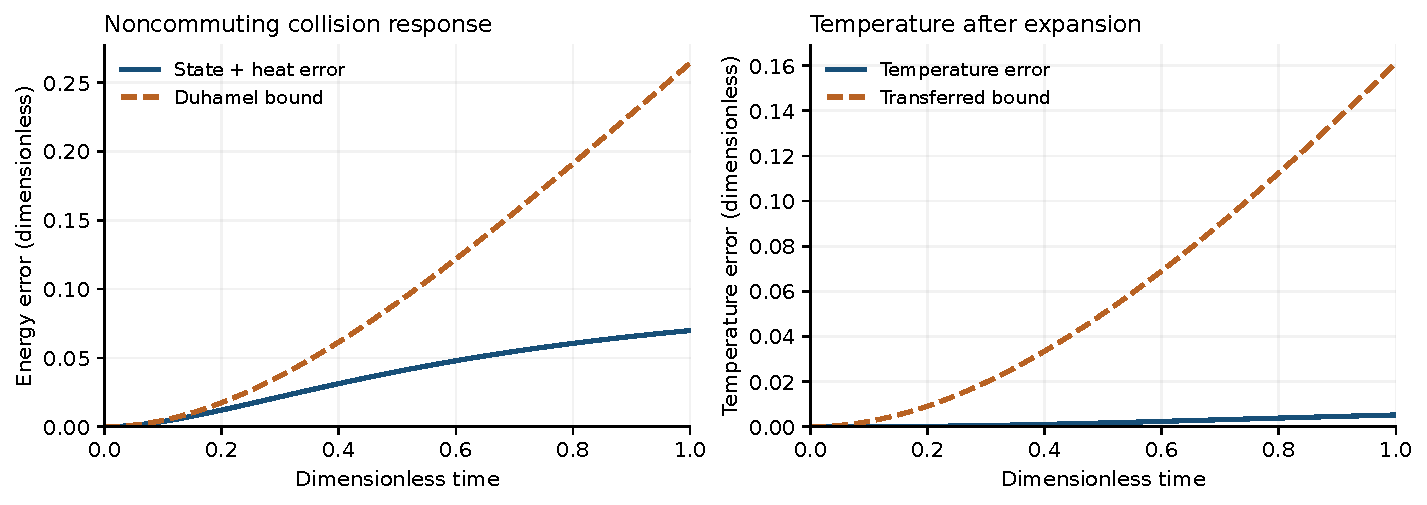
\includegraphics[width=\linewidth]{../figures/theory_certificates.pdf}
\caption{비가환 두 채널의 새 판별 예제. 왼쪽은 state와 누적 heat 오차, 오른쪽은 팽창 후 thermal temperature 오차다. 실선은 저장된 수치 결과, 점선은 증명에서 계산한 상계다.}
\end{figure}

column 최대값과 입력 energy envelope를 사용한 상계에는 여유가 있다. observable별로 더 작은 상계가 필요하면 이미 유도한 Duhamel 잔차의 \(\Delta\widehat X\) 또는 output sensitivity를 사용하면 된다. 이는 더 필요한 입력과 직접 연결되는 개선 경로다.

\hypertarget{uxb3c5uxb9bd-uxac80uxd1a0uxc5d0uxc11c-uxc218uxc815uxd55c-uxc0acuxd56d}{%
\subsection{독립 검토에서 수정한 사항}\label{uxb3c5uxb9bd-uxac80uxd1a0uxc5d0uxc11c-uxc218uxc815uxd55c-uxc0acuxd56d}}

검토자는 후보 유도와 root의 계산을 작성하지 않은 별도 분과로 두었다. moving boundary에는 Heaviside 분포 미분, all-free에는 exact inverse substitution, 잔차에는 positive propagator와 Duhamel 식, clock 선택에는 convex subgradient를 사용했다. 수정된 항목은 다음과 같다.

\begin{enumerate}
\def\labelenumi{\arabic{enumi}.}
\tightlist
\item
  \(P_h\)의 정의를 continuous stopping과 선언한 직접 jump heat의 합으로 통일하고, 전체 medium debit에서 chemical/excitation 항을 분리했다.
\item
  SI energy state를 입력으로 받는 number row에 \(1/(T_0\epsilon_{\rm eV})\)를 명시했다. 전체 mixed state에는 대각 similarity transform을 썼다.
\item
  weighted median을 양의 허용 clock 구간으로 projection하고, source shape의 비음 조건과 zero-weight 경우를 명시했다.
\item
  저장 cutoff 총량에 포함된 source ghost를 한 번만 사용하는 대응식을 유지했다.
\end{enumerate}

\hypertarget{uxc2dduxc5d0uxc11c-uxcf54uxb4dcuxb85c-uxc62euxae34-uxacb0uxacfc}{%
\section{식에서 코드로 옮긴 결과}\label{uxc2dduxc5d0uxc11c-uxcf54uxb4dcuxb85c-uxc62euxae34-uxacb0uxacfc}}

작은 receiver 모듈은 순수 Python으로 작성했으며, 정확한 유리수 입력을 float로 강제 변환하지 않는다. 기본 \(k_B\)는 정확한 SI 값이다.

\begin{longtable}[]{@{}
  >{\raggedright\arraybackslash}p{(\columnwidth - 2\tabcolsep) * \real{0.5000}}
  >{\raggedright\arraybackslash}p{(\columnwidth - 2\tabcolsep) * \real{0.5000}}@{}}
\toprule\noalign{}
\begin{minipage}[b]{\linewidth}\raggedright
함수
\end{minipage} & \begin{minipage}[b]{\linewidth}\raggedright
입력과 역할
\end{minipage} \\
\midrule\noalign{}
\endhead
\bottomrule\noalign{}
\endlastfoot
thermal\_transfer\_tdot & thermal 수·energy 전달과 expansion으로 \(\dot T\) 계산 \\
total\_moment\_tdot & total source와 active 모멘트에서 동일한 thermal 식을 구성 \\
advance\_thermal\_packet & 적분된 comoving 수·energy를 더하고 EOS inversion \\
temperature\_error\_bound & endpoint energy·number certificate를 온도 상계로 전달 \\
\end{longtable}

source와 전달률을 같은 시각·부피·단위로 입력하도록 docstring에 정의했다. positive thermal count, physical endpoint energy, finite inputs를 확인한다. 실제 time integrator에 연결할 때는 수·energy·pressure work를 같은 step의 적분량으로 공급한다.

\hypertarget{uxc774uxb860-uxb8e8uxd504uxc758-uxd310uxc815uxacfc-uxc774uxc5b4uxac08-uxc5f0uxad6c}{%
\section{이론 루프의 판정과 이어갈 연구}\label{uxc774uxb860-uxb8e8uxd504uxc758-uxd310uxc815uxacfc-uxc774uxc5b4uxac08-uxc5f0uxad6c}}

이번 R1--R10은 근거 복원, 가정 정리, 후보식 구성, 실제 유도, 독립 검토, 판별 계산, 결과 판정, 코드 인터페이스와 원고, 다음 DAG까지 진행했다. 명시한 조건의 보존식·변수변환·잔차 정리는 이번 연구의 완료 결과다.

다음 이론 루프의 중심은 \textbf{온도와 이온화 조성이 collision coefficients에 되먹임되는 계를 양수성과 수·energy 보존을 유지하면서 한 step으로 연결하는 구성}이다. 현재 결과를 그대로 사용하면 작업 순서는 구체적이다.

\begin{enumerate}
\def\labelenumi{\arabic{enumi}.}
\tightlist
\item
  고정된 반응별 energy-transfer 행렬에 \(n_e(t)\), \(n_{\rm HI}(t)\), \(n_{\rm HeI}(t)\)와 thermal variables의 coefficient를 결합한다.
\item
  active state, chemical count, thermal energy를 함께 갱신하는 conservative positive step을 구성한다.
\item
  현재 Coulomb residual과 source mismatch를 사용해 step 안의 coefficient 변화 오차를 제한한다.
\item
  fixed cutoff에서 시작하고, 필요한 경우 이번 signed interface와 하부 trace로 moving cutoff를 결합한다.
\item
  선택된 실제 scenario에는 initial stock, source history, background와 원하는 observable budget를 입력한다.
\end{enumerate}

현재 실제 응용의 scenario·receiver 채택 노드와 원래의 전역 연구 상태는 각각 보존했다. DAG에는 이번에 완료한 이론 노드와 그것을 사용하는 다음 구성을 추가했다. 새 NCP 작업이나 대규모 원자·transport 계산은 이 연구 단위에 필요하지 않았다.

\hypertarget{uxcd9cuxcc98uxc640-uxc7acuxd604-uxc790uxb8cc}{%
\section{출처와 재현 자료}\label{uxcd9cuxcc98uxc640-uxc7acuxd604-uxc790uxb8cc}}

직전 DERIVATION\_KO.md §4, §6.1--§6.4와 SOURCE\_BOUND\_RESPONSE.json을 inputs/prior에 포함했다. 원 causal\_cascade.py는 source identity를 유지하여 inputs/prior\_code에 보관했다. 세 유도문, 검산 코드·기호 스크립트·실행 결과, independent review, CONTRACT, NEXT\_DAG와 PLAN을 같은 묶음에 제공한다.

전체 계산은 checks/run\_theory\_checks.py로 재현할 수 있다. 이 명령은 이번의 15개 focused checks와 작은 IVP만 수행한다. Wolfram의 정확한 두 단계 예제는 checks/verify\_analytic\_case.wl에 따로 제공한다. PDF는 LaTeX 원고와 포함한 font·figure로 다시 컴파일할 수 있다.

\begin{thebibliography}{9}
\bibitem{prior}
BASS\_CR, \emph{실제 전자 birth source와 M0 응답의 정규화 결속},
CR-RUX-M1B-SOURCE-BINDING-20261012, science commit 5fc11143679f.
보존 원문과 결과: 이 묶음의 inputs/prior.
\bibitem{cascade}
BASS\_CR, \emph{causal\_cascade.py}, CR-PHYS02B.
SHA-256 d87a9cc12212\ldots f39313c7b72.
stopping, project, generator와 moment functionals.
\bibitem{sz}
O. Sarbach and T. Zannias,
\emph{Relativistic Kinetic Theory: An Introduction} (2013).
\url{https://arxiv.org/abs/1303.2899}.
Proposition 6, Eqs. (62)–(63), collision moment Eq. (76).
\bibitem{ln}
H. Lee and E. Nungesser,
\emph{Bianchi I solutions of the Einstein--Boltzmann system with a positive cosmological constant}.
\url{https://arxiv.org/abs/1705.07009}.
직교기저 §1.1, Bianchi I의 kinetic moments §3.
\bibitem{soderlind}
G. Söderlind,
\emph{The logarithmic norm. History and modern theory},
BIT Numerical Mathematics 46, 631--652 (2006).
\url{https://doi.org/10.1007/s10543-006-0069-9}.
서지·abstract를 확인한 방법론 배경이며 본문의 inequality는 직접 증명했다.
\end{thebibliography}

\end{document}
